% $Header: /home/vedranm/bitbucket/beamer/solutions/conference-talks/conference-ornate-20min.en.tex,v 90e850259b8b 2007/01/28 20:48:30 tantau $

\documentclass{beamer}

\mode<presentation>
{
  \usetheme{Rochester}
  % or ...

  \setbeamercovered{transparent}
  \addtobeamertemplate{navigation symbols}{}{%
    \usebeamerfont{footline}%
    \usebeamercolor[fg]{footline}%
    \hspace{1em}%
    \insertframenumber
}
}

\usepackage{graphicx}
\usepackage{mathdots}
\usepackage[english]{babel}

\usepackage[latin1]{inputenc}

\usepackage{times}
\usepackage[T1]{fontenc}
\usepackage{array}
\usepackage{mathtools}

\usefonttheme[onlymath]{serif}


% To create new paragraphs
% \setlength{\parindent}{0em}
% \setlength{\parskip}{1em}

\newcommand{\bunderline}[1]{\underline{#1}}
\renewcommand{\vec}[1]{{\bunderline{#1}}}
\newcommand{\vect}[1]{{\bunderline{#1}}} 
\newcommand{\mat}[1]{{\bunderline{\bunderline{#1}}}}

\renewcommand{\arraystretch}{1.5}
\setbeamercovered{invisible}

\title[Solving the Radiative Transfer Equation via the Radon Transform] 
{Solving the Radiative Transfer Equation \\ via the Radon Transform}

\author[Nelluvelil, Oeltjenbruns, Spainhour]
{E. Nelluvelil \inst{1} \and M. Oeltjenbruns \inst{2} \and J. Spainhour \inst{3}}

\institute[Iowa State University] 
{
  \,\,\,\, \inst{1} \, Rice University \quad \quad
  \inst{2} \, Wayne State College \quad \quad
  \inst{3} \, Florida State University }
  

\date[ISU REU 2019] 
{Modeling and Computation Group \\
	ISU Math REU 2019}
	
\logo{
    
\includegraphics[width=1.85cm,height=1.85cm,keepaspectratio]{figures/NSF.png}
    \hspace{\dimexpr\paperwidth-4cm-15pt}
    
\includegraphics[width=2cm,height=2cm,keepaspectratio]{figures/logo.jpg}
    \hspace{5pt}
}
%\AtBeginSection[]
\AtBeginSubsection[]
{
  \begin{frame}<beamer>{Outline}
    \tableofcontents[currentsection,currentsubsection]
  \end{frame}
}

%\beamerdefaultoverlayspecification{<+->}


\begin{document}

\begin{frame}
  \titlepage
\end{frame}

\logo{}

\begin{frame}{Outline}
  \tableofcontents
\end{frame}

\section{Motivation}

\subsection*{Goal}

\begin{frame}{Imaging Problem}
    \begin{itemize}
        \item
            The imaging problem is to reconstruct a distribution from several profiles taken at different angles
        \item
            The Radon transform is a simple way to produce profiles
    \end{itemize}
    
    \begin{figure}[H]
    \centering
    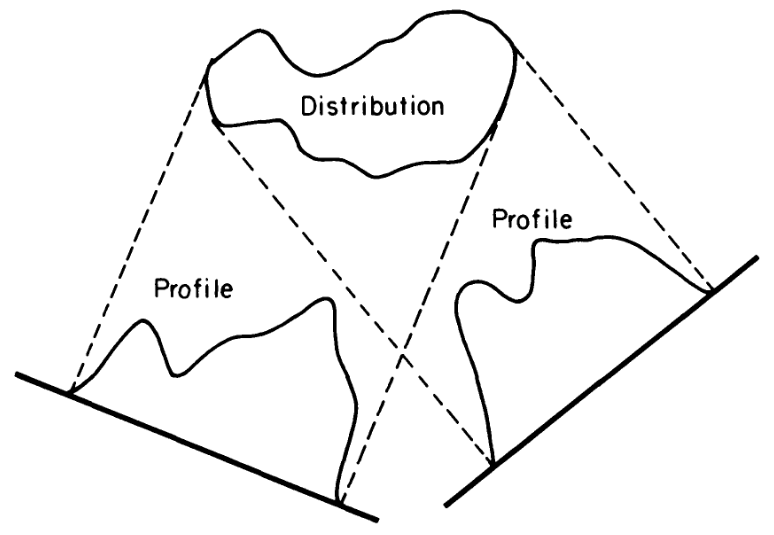
\includegraphics[width=0.5\textwidth]{figures/profiles.png}
    \\ \scriptsize Deans, S. (1983) \textit{The Radon Transform and Some of Its Applications}. Wiley-Interscience Publication. 1983. Pg 3.
    \end{figure}
    
    \begin{itemize}
        \item
            Certain advection problems are easier to solve profile-by-profile
    \end{itemize}    
\end{frame}

\begin{frame}{Our Goal}
    \begin{itemize}
        \item
            To efficiently solve multi-dimensional systems of hyperbolic partial differential equations using the Radon transform
            \\ \color{white} hi \color{black} \\
        \item
            Three main steps:
        \begin{enumerate}
            \item
                Forward Radon transform multi-dimensional problem
            \item
                Solve family of 1D advection problems 
            \item
                Use inverse Radon transform to original space
        \end{enumerate}
    \end{itemize}
\end{frame}

\begin{frame}{Notation}
    \begin{itemize}
        \item
            We will use the following notation in the presentation:
%        \begin{itemize}
%            \item $\mathcal{R}$ refers to the Radon transform
%            \item Hats denote the Radon transform of a function (e.g. $\mathcal{R} \, (f) := \widehat{f}$) 
%            \item Underlines denote vectors (e.g. $\vec{v}$)
%            \item Double underlines denote matrices (e.g. $\mat{A}$)
%            \item Comma subscripts on functions followed by a variable refer to a partial derivative (e.g $\frac{\partial}{\partial t} \, f := f_{, t}$)
%            \item \textbf{Note}: Put this in table form for readability
%        \end{itemize}
    \end{itemize}
    \begin{center}
        \begin{tabular}{| c | c |}
        \hline
        Radon transform & $\mathcal{R}$ \\
        \hline
        Radon transform of a function & $\widehat{f}$ \\
        \hline
        Vector & $\vec{v}$ \\
        \hline
        Matrix & $\mat{A}$ \\
        \hline
        Partial derivative & $f_{, t}$ \\
        \hline
        \end{tabular}
    \end{center}
\end{frame}

\section{The Radon Transform}
\subsection{Radon Transform Derivation in 2D}

\begin{frame}{Coordinate Transform}
\begin{itemize}
    \item
        To get a single profile, rotate the $xy$ coordinate system by a positive angle $\omega$ to obtain the $sz$ coordinate system using a rotation matrix:
    %\item
    %    We can write each point $(x, y)$ in terms of $s$, $z$, and $\omega$ using the following rotation matrix:
        \begin{align*}
            \begin{bmatrix}
                x \\
                y
            \end{bmatrix}
            & = 
            \begin{bmatrix}
                \cos (\omega) & -\sin (\omega) \\
                \sin (\omega) & \cos (\omega)
            \end{bmatrix}
            \begin{bmatrix}
                s \\
                z
            \end{bmatrix} \\
        \end{align*}
    \pause
    \item
        Use the inverse of the matrix to obtain the reverse transform:
        \begin{align*}
            \begin{bmatrix}
                s \\
                z
            \end{bmatrix}
            & = 
            \begin{bmatrix}
                \cos (\omega) & \sin (\omega) \\
                 -\sin (\omega) & \cos (\omega)
            \end{bmatrix}
            \begin{bmatrix}
                x \\
                y
            \end{bmatrix}
        \end{align*}
\end{itemize}
\end{frame}

\begin{frame}{Coordinate Rotation}
	\begin{figure}[H] 
		\centering %% This plot needs labels
		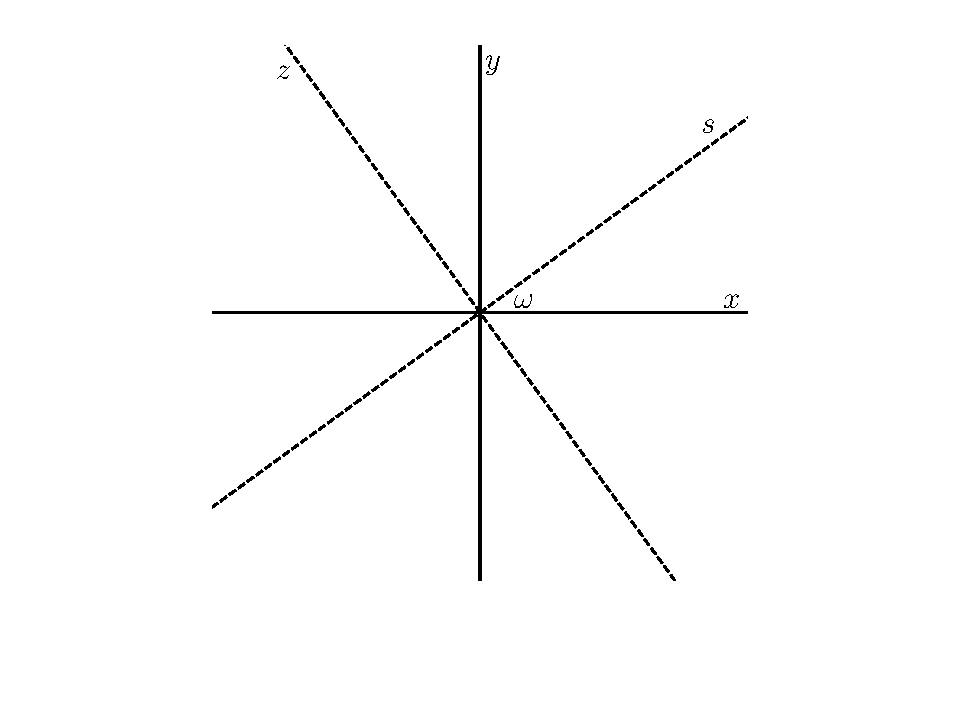
\includegraphics[width=0.8\linewidth]{figures/rotation1.pdf}
		% \caption{$xy$ coordinate system and unit circle}
		\label{fig:xy_unit_circle_s_z}
	\end{figure}
\end{frame}

\begin{frame}{Coordinate Transform}
\begin{itemize}
    \item
        Rewrite the rotation matrices: % Mention helpful for derivatives
    \begin{align*}
        x(s, z; \omega) & = s\, \cos (\omega) - z\,\sin (\omega) \\
        y(s, z; \omega) & = s\, \sin (\omega) + z\,\cos (\omega) \\
        s(x, y; \omega) & = x \cos (\omega) + y \sin (\omega) \\
        z(x, y; \omega) & = -x \sin (\omega) + y \cos (\omega)
    \end{align*}
    \item
        To construct a single profile, $\omega$ is constant
\end{itemize}
\end{frame}

\begin{frame}{Radon Transform}
\begin{itemize}
    \item
        Suppose $f: \mathbb{R}^{2} \rightarrow \mathbb{R}$ is a function with compact support % Define compact support
    \item
        After rotating by $\omega$, select a point on the new $s$-axis and integrate parallel to the new $z$-axis
    \item
        The Radon transform of $f$ is formally defined as follows
    %\int_{-\infty}^{\infty} \int_{-\infty}^{\infty} \, f(x, y) \, \delta (x \cos (\omega) + y \sin (\omega) - s) \, dx \, dy \\
    \begin{align*}
        \mathcal{R}(\,f) = \widehat{f}(s, \omega) & := \int_{-\infty}^{\infty} f(\,x(s, z;\omega), y(s, z;\omega)\,) \, dz \\
                              & = \int_{-\infty}^{\infty} f(s \cos (\omega) - z \sin (\omega), s \sin (\omega) + z \cos (\omega)) \, dz
    \end{align*}
    \item $\mathcal{R}$ is a linear operator
\end{itemize}
\end{frame}

%\begin{frame}{Radon Transform at $(s_0, \omega_0)$}
%	\begin{figure}[H] 
%		\centering %% This plot needs labels
%		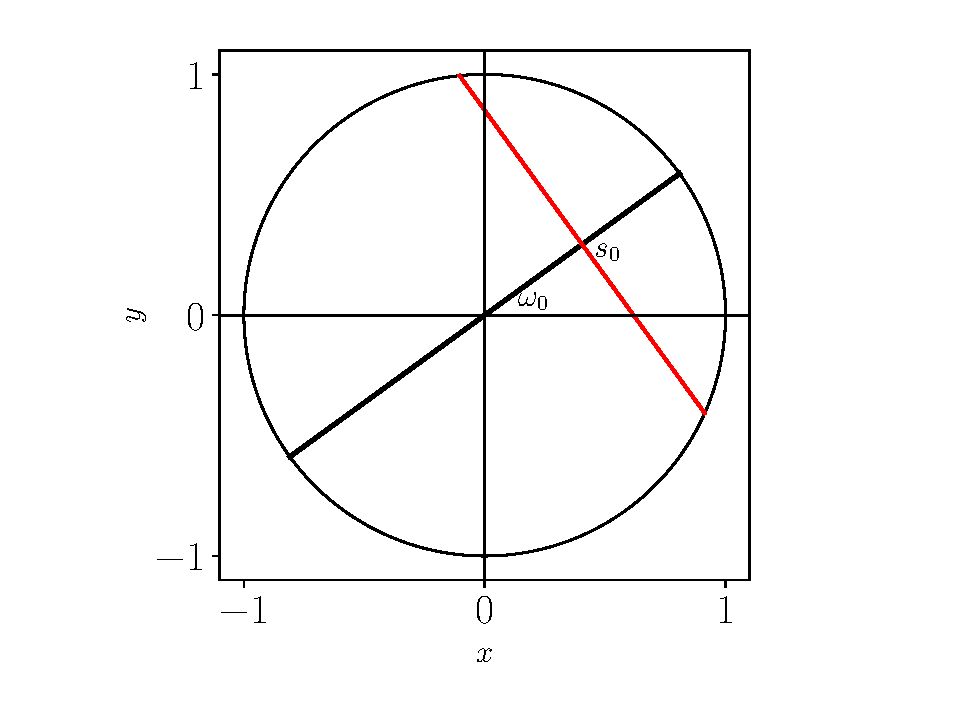
\includegraphics[scale=0.55]{figures/unit_circle.pdf}
%		% \caption{$xy$ coordinate system and unit circle}
%		%\label{fig:xy_unit_circle_s_z}
%	\end{figure}
%\end{frame}

\begin{frame}{Radon Transform at $(x_0, y_0)$}
	\begin{figure}[H]
		\centering
		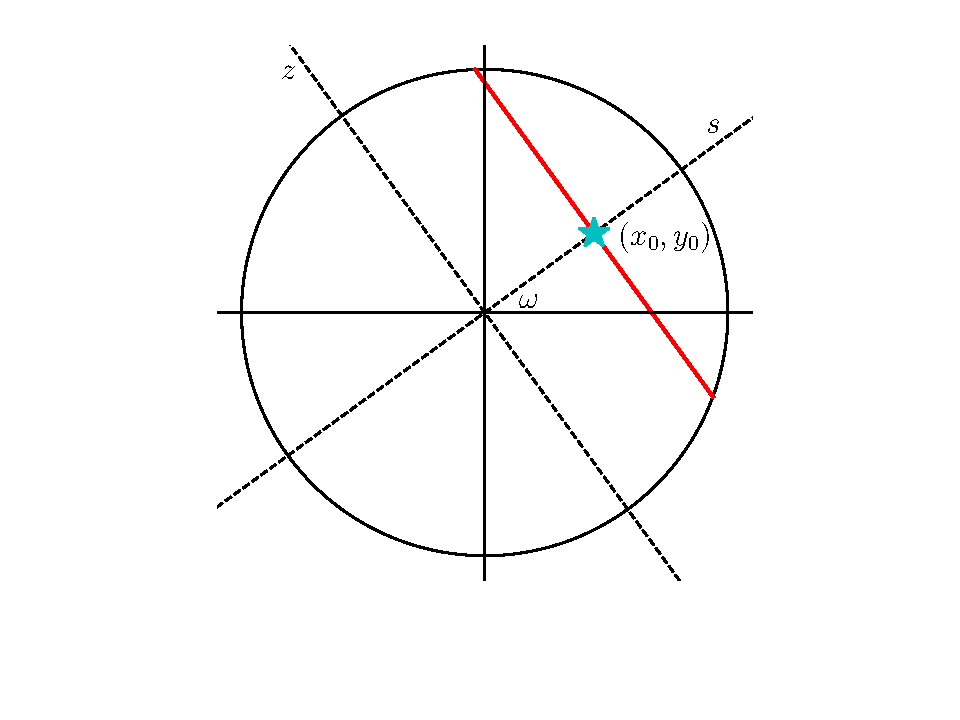
\includegraphics[scale=0.65]{figures/Radon.pdf}
	\end{figure}
\end{frame}

\begin{frame}{Radon Transform}
	\begin{figure}[H]
		\centering
		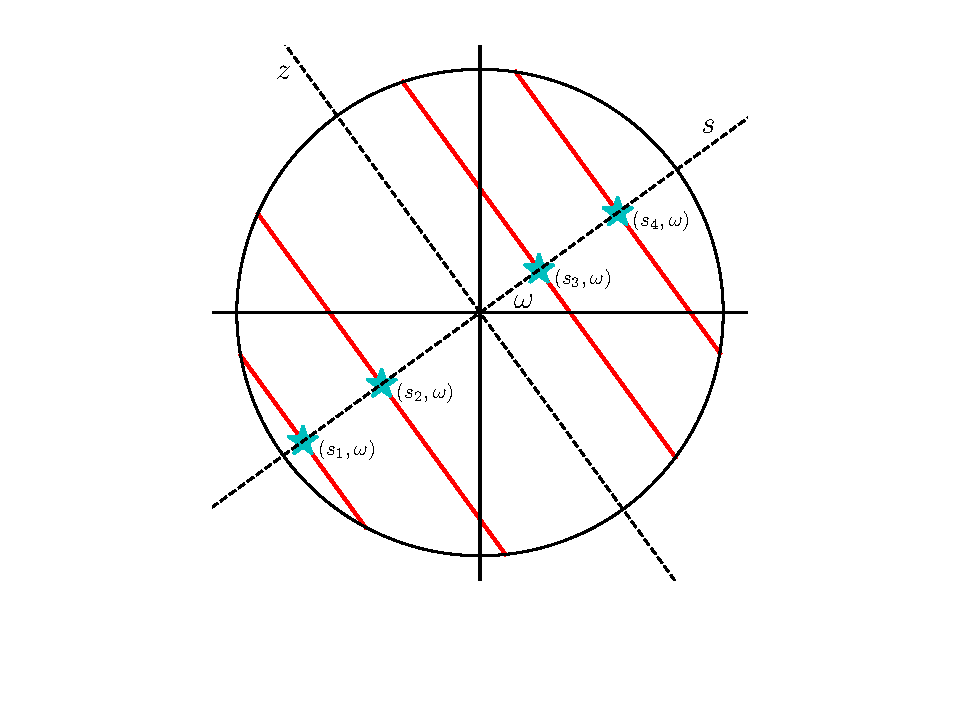
\includegraphics[scale=0.65]{figures/AllRadon.pdf}
	\end{figure}
\end{frame}

\begin{frame}{Radon Transform Example}
    \hspace{-0.1\linewidth}
    \begin{minipage}[r]{0.5\linewidth}
        \begin{figure}[r]
            \centering
            \makebox[\textwidth][c]{
            	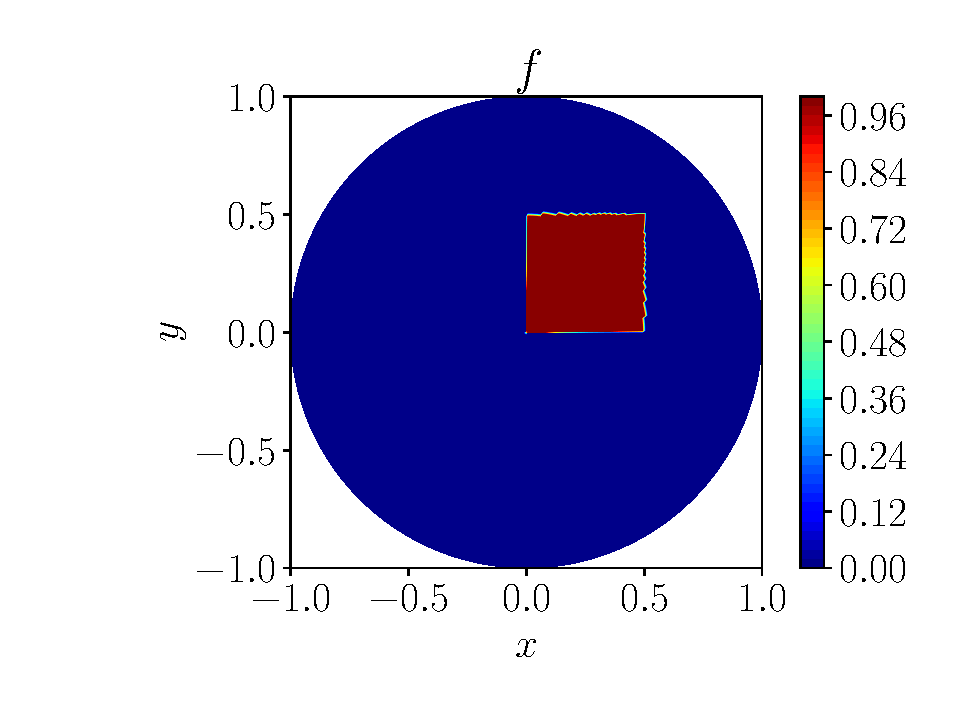
\includegraphics[height=5cm]{figures/unit_square_physical.pdf}}
        \end{figure}    
    \end{minipage}
    \hspace{0.3cm}
    \begin{minipage}[c]{0.1\linewidth}
        \begin{figure}[c]
            \centering
            \makebox[\textwidth][l]{                       	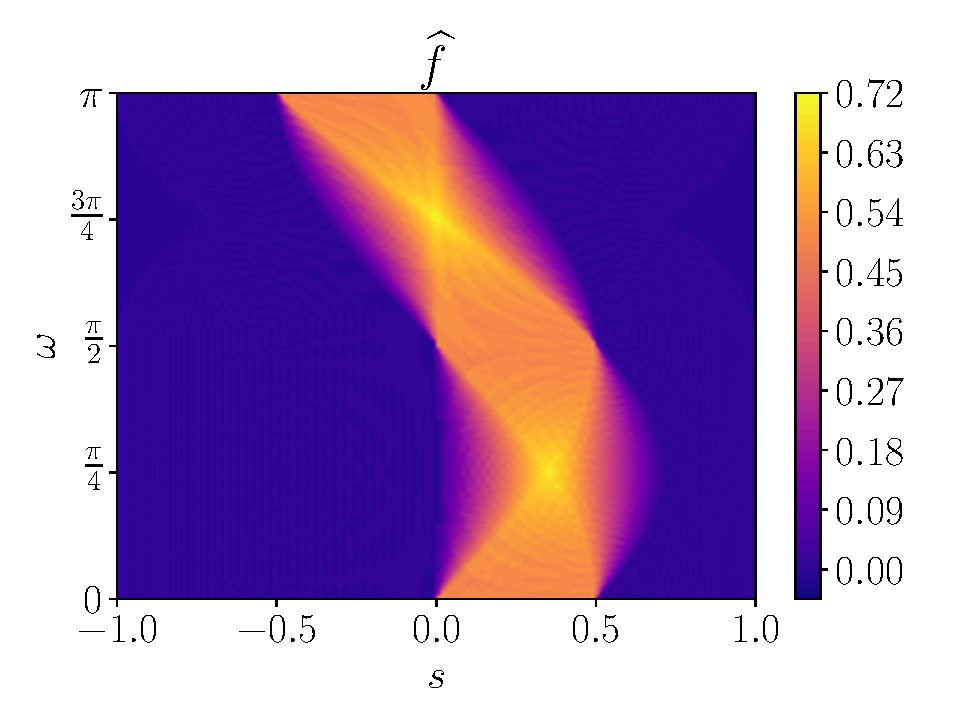
\includegraphics[height=4.5cm]{figures/unit_square_radon.pdf}}
        \end{figure}
    \end{minipage}
\end{frame}

\begin{frame}{Radon Transform Example}
	\hspace{-0.1\linewidth}
	\begin{minipage}[r]{0.5\linewidth}
		\begin{figure}[r]
			\centering
			\makebox[\textwidth][c]{
				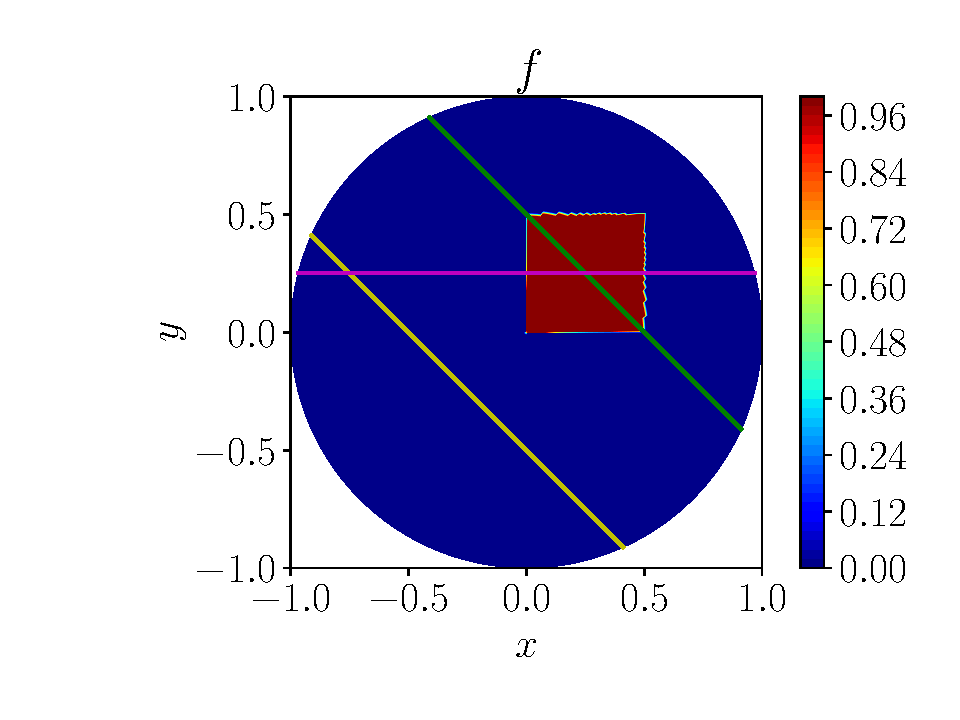
\includegraphics[height=5cm]{figures/unit_square_physical_slices.pdf}}
		\end{figure}    
	\end{minipage}
	\hspace{0.3cm}
	\begin{minipage}[c]{0.1\linewidth}
		\begin{figure}[c]
			\centering
			\makebox[\textwidth][l]{                       	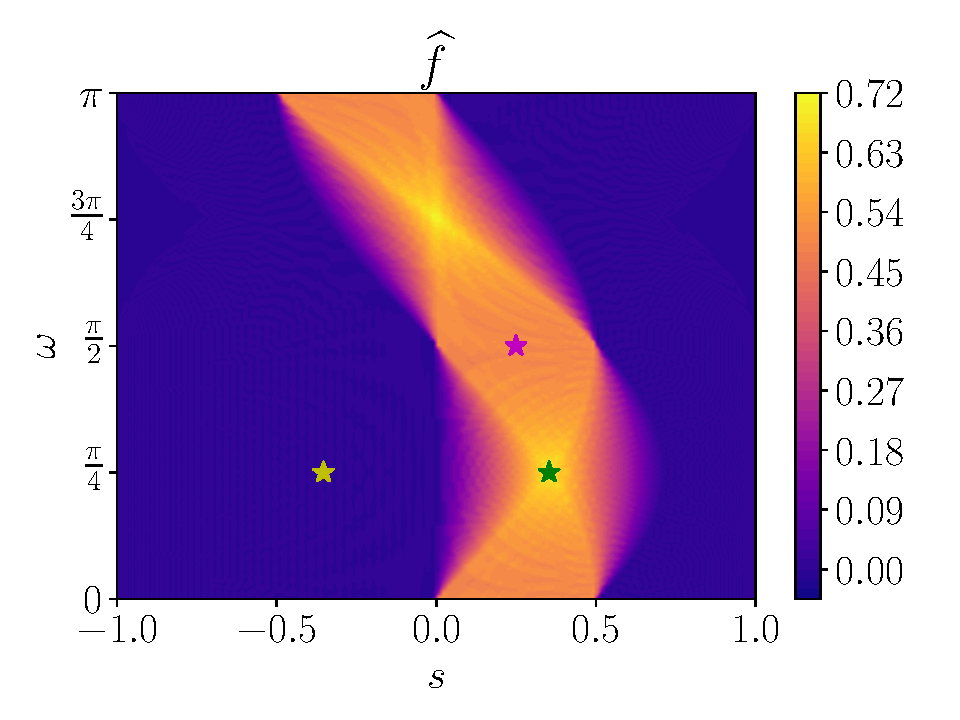
\includegraphics[height=4.5cm]{figures/unit_square_radon_slices.pdf}}
		\end{figure}
	\end{minipage}
\end{frame}

\subsection{Discretizing the Radon Transform}

\begin{frame}{Grid Structure}
\begin{itemize}
    \item
        Need discretized domain for inverse computation
    \item
        Profile-by-profile construction suggests $N_\omega$ evenly-spaced diameters
    \item
        Along each diameter, create $N_s$ Chebyshev points of the second kind:
    \begin{align*}
        s_j = \cos \left( \frac{j\pi}{N_s} \right) \quad \text{for $j = 0, 1, \dots, N_s$}
    \end{align*}
    \begin{itemize}
        \item Allows for spectrally accurate interpolation, differentiation
        %\item A spectrally accuarate method is one for which the error rapidly tends to zero when applied to smooth functions.
    \end{itemize}
\end{itemize}
\end{frame}

\begin{frame}{Grid Structure Example}
    \begin{figure}[H]
        \centering
        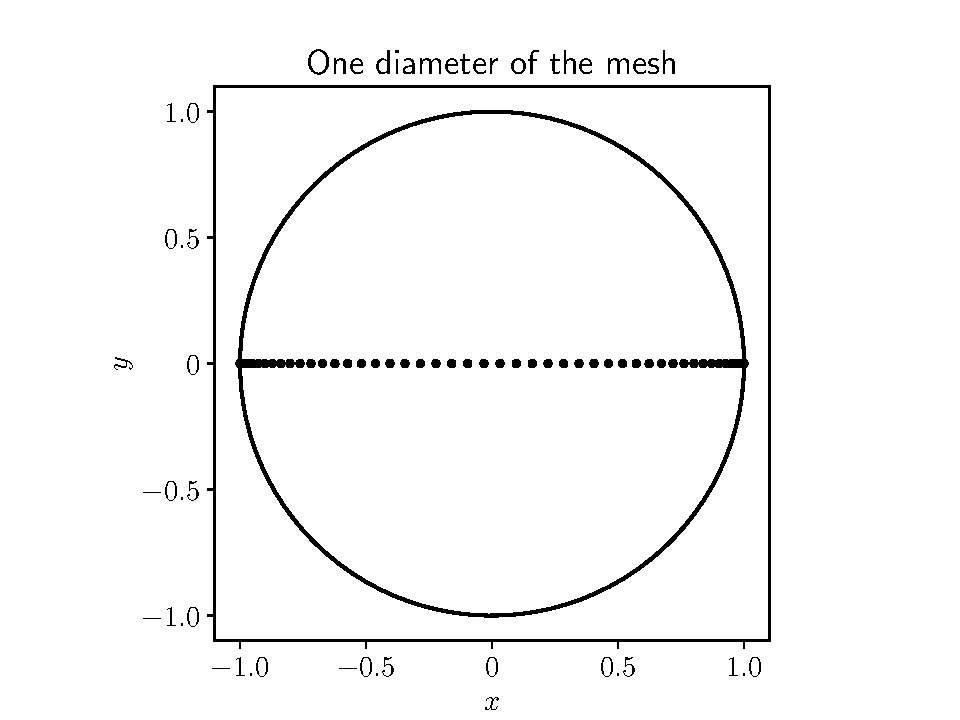
\includegraphics[scale=0.55]{figures/one_diameter.pdf}
        %\label{fig:one_diameter}
    \end{figure}
\end{frame}

\begin{frame}{Grid Structure Example}
    \begin{figure}[H]
        \centering
        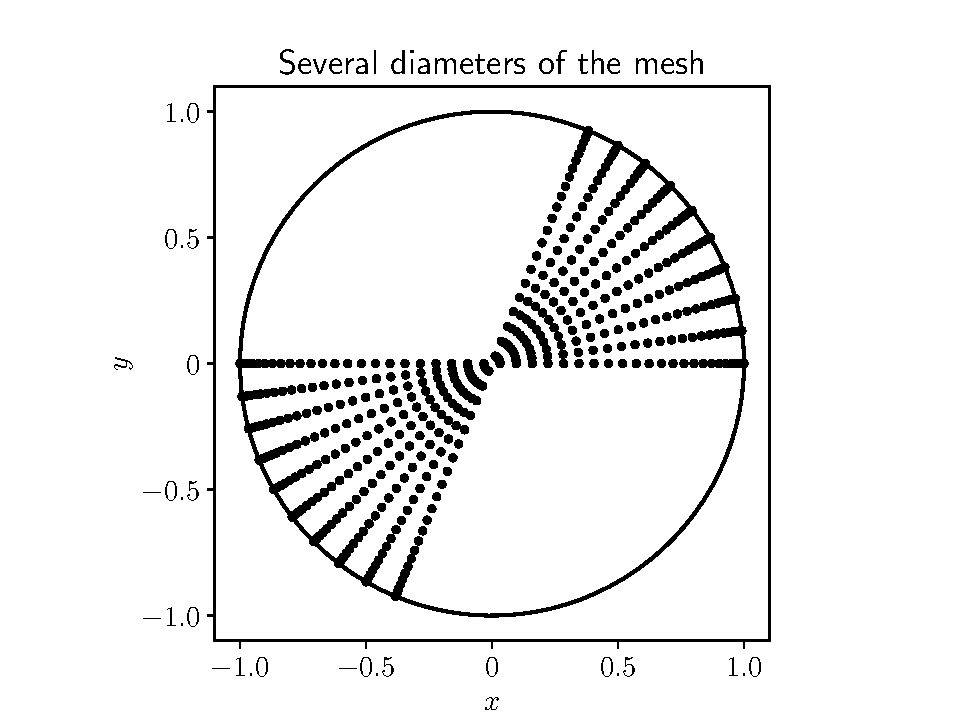
\includegraphics[scale=0.55]{figures/several_diameters.pdf}
        %\label{fig:several_diameters}
    \end{figure}
\end{frame}

\begin{frame}{Grid Structure Example}
    \begin{figure}[H]
        \centering
        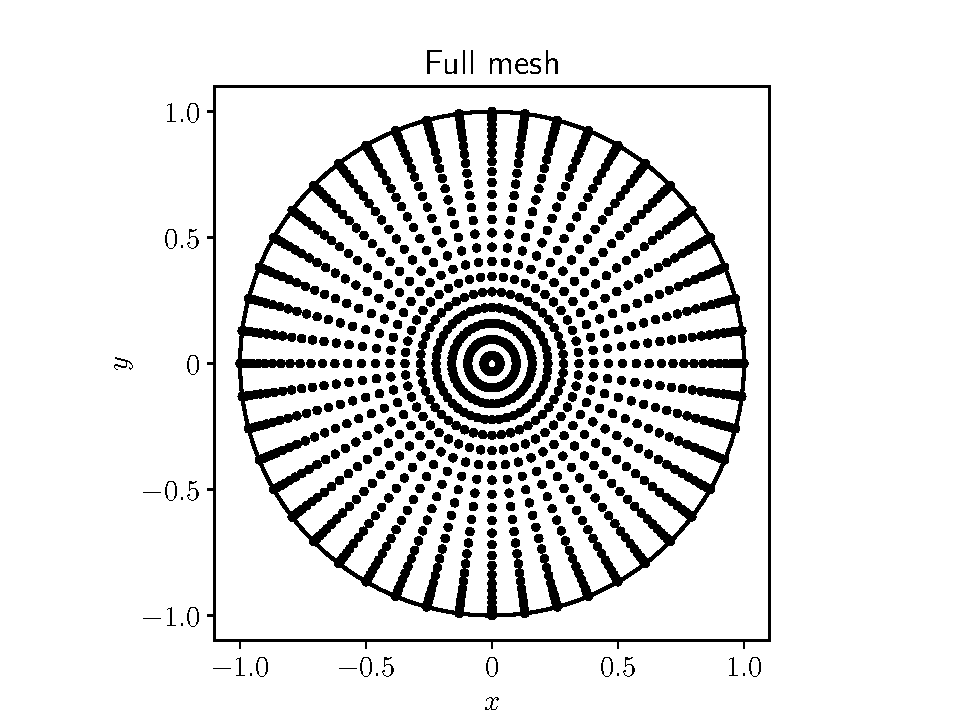
\includegraphics[scale=0.55]{figures/full_mesh.pdf}
        %\label{fig:full_mesh}
    \end{figure}
\end{frame}

\begin{frame}{Computing Integrals}
    \begin{itemize}
        \item
            Compact support of $f$ means we compute line integrals across chords of the domain
        \item
            Compute line integrals with Clenshaw-Curtis quadrature
    \end{itemize}
    \begin{align*}
    	\mathcal{R}(\,f) &= \int_{-\infty}^{\infty} f(x, y) \, dz\\ &= \int_{-\tau}^{\tau} f(x, y) \, dz\\ &\approx \sum_{i=1}^{N_q} w_{i} \, f(z_{i})
    \end{align*}
\end{frame}

\begin{frame}{Quadrature Example}
	\begin{figure}[H]
		\centering
		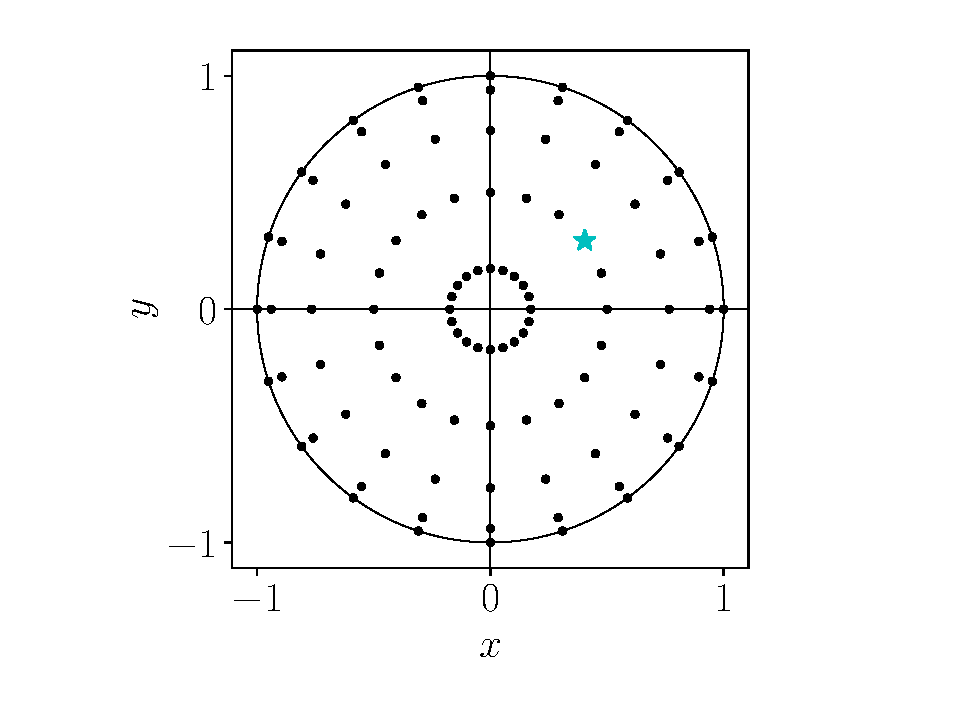
\includegraphics[scale=0.65]{figures/quad_1.pdf}
		%\label{fig:full_mesh}
	\end{figure}
\end{frame}

\begin{frame}{Quadrature Example}
	\begin{figure}[H]
		\centering
		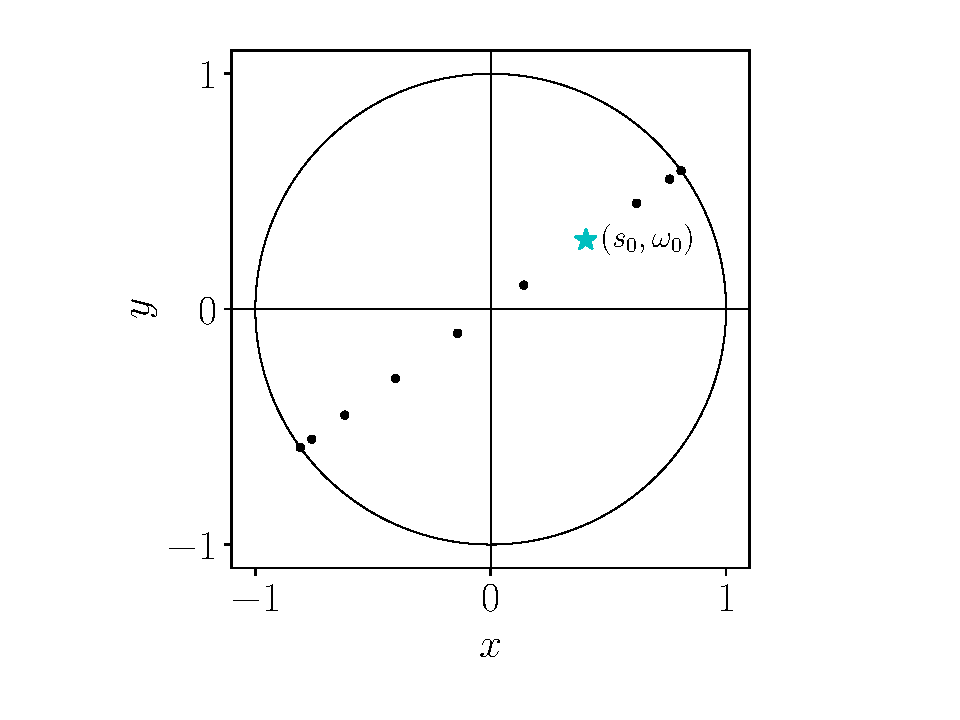
\includegraphics[scale=0.65]{figures/quad_2.pdf}
		%\label{fig:full_mesh}
	\end{figure}
\end{frame}

\begin{frame}{Quadrature Example}
	\begin{figure}[H]
		\centering
		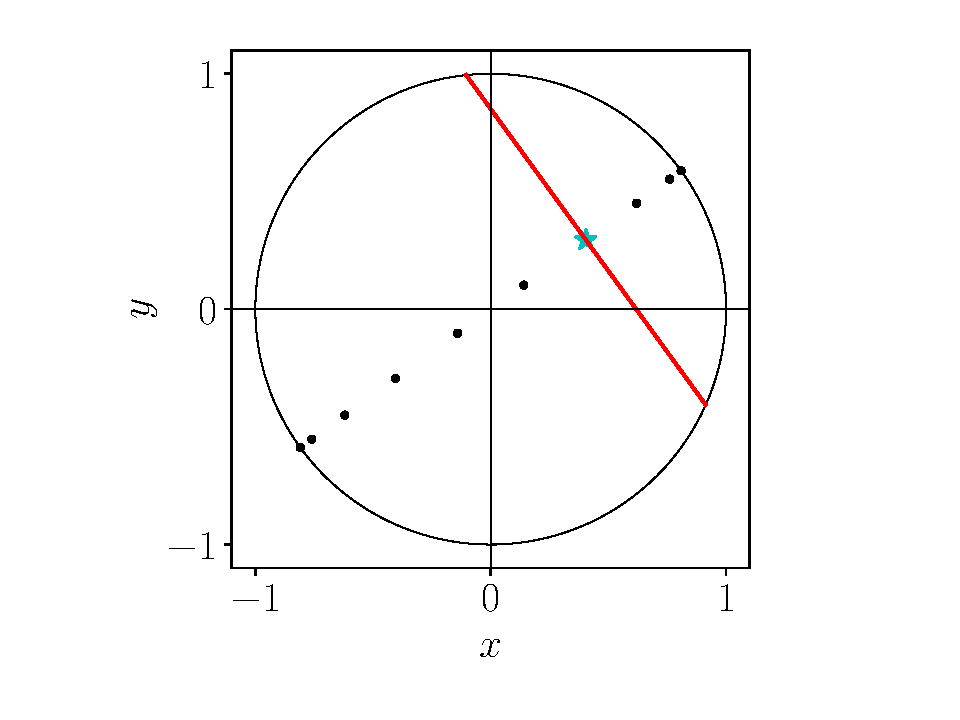
\includegraphics[scale=0.65]{figures/quad_3.pdf}
		%\label{fig:full_mesh}
	\end{figure}
\end{frame}

\begin{frame}{Quadrature Example}
	\begin{figure}[H]
		\centering
		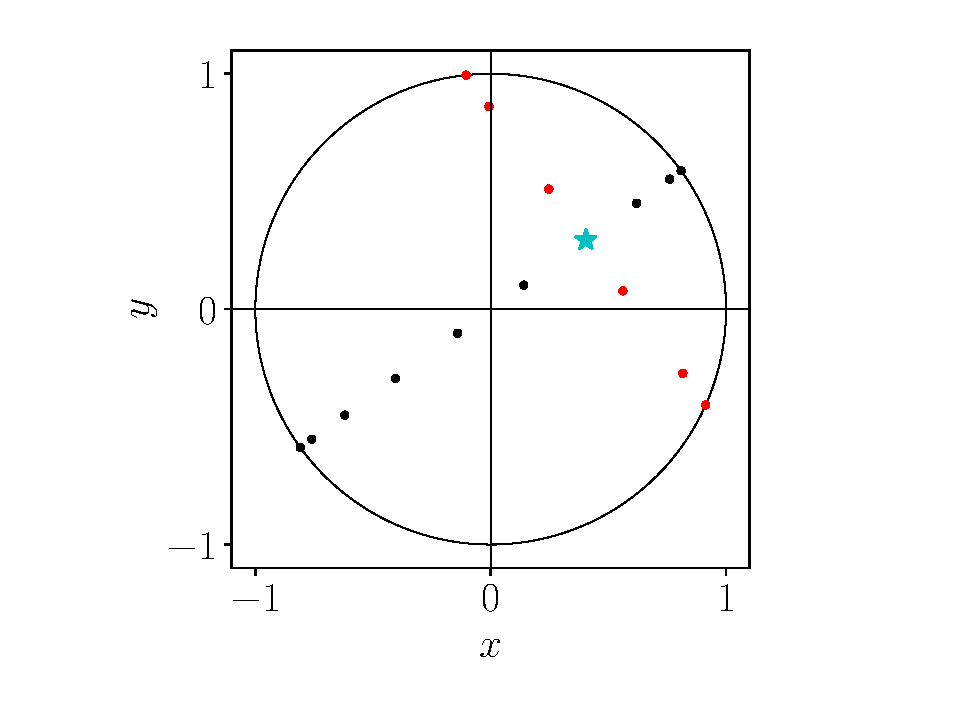
\includegraphics[scale=0.65]{figures/quad_4.pdf}
		%\label{fig:full_mesh}
	\end{figure}
\end{frame}

\begin{frame}{Quadrature Example}
	\begin{figure}[H]
		\centering
		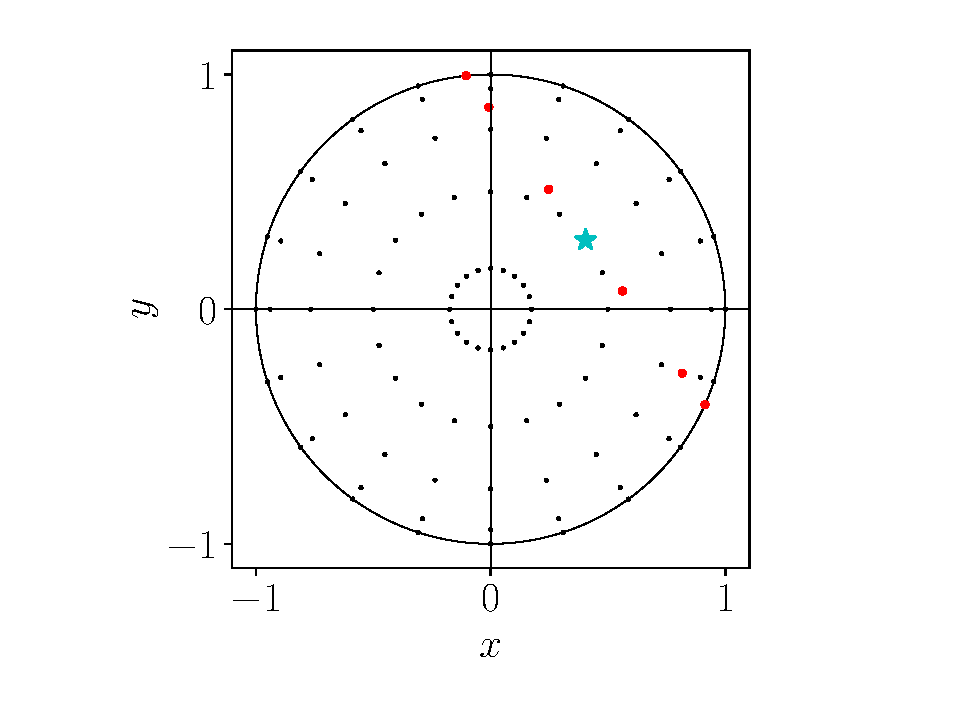
\includegraphics[scale=0.65]{figures/quad_5.pdf}
		%\label{fig:full_mesh}
	\end{figure}
\end{frame}

\begin{frame}{Interpolation Scheme}
    \begin{itemize}
        \item
            Need to sample $f$ at arbitrary quadrature nodes, use interpolation
        \item
            Use a series of one-dimensional interpolation schemes:
        \begin{itemize}
            \item
                Spectrally accurate on each diameter
            \item
                Fourth order accurate across angles
        \end{itemize}
    \end{itemize}
\end{frame}

\begin{frame}{Interpolation Scheme Example}
	\begin{figure}[H]
		\centering
		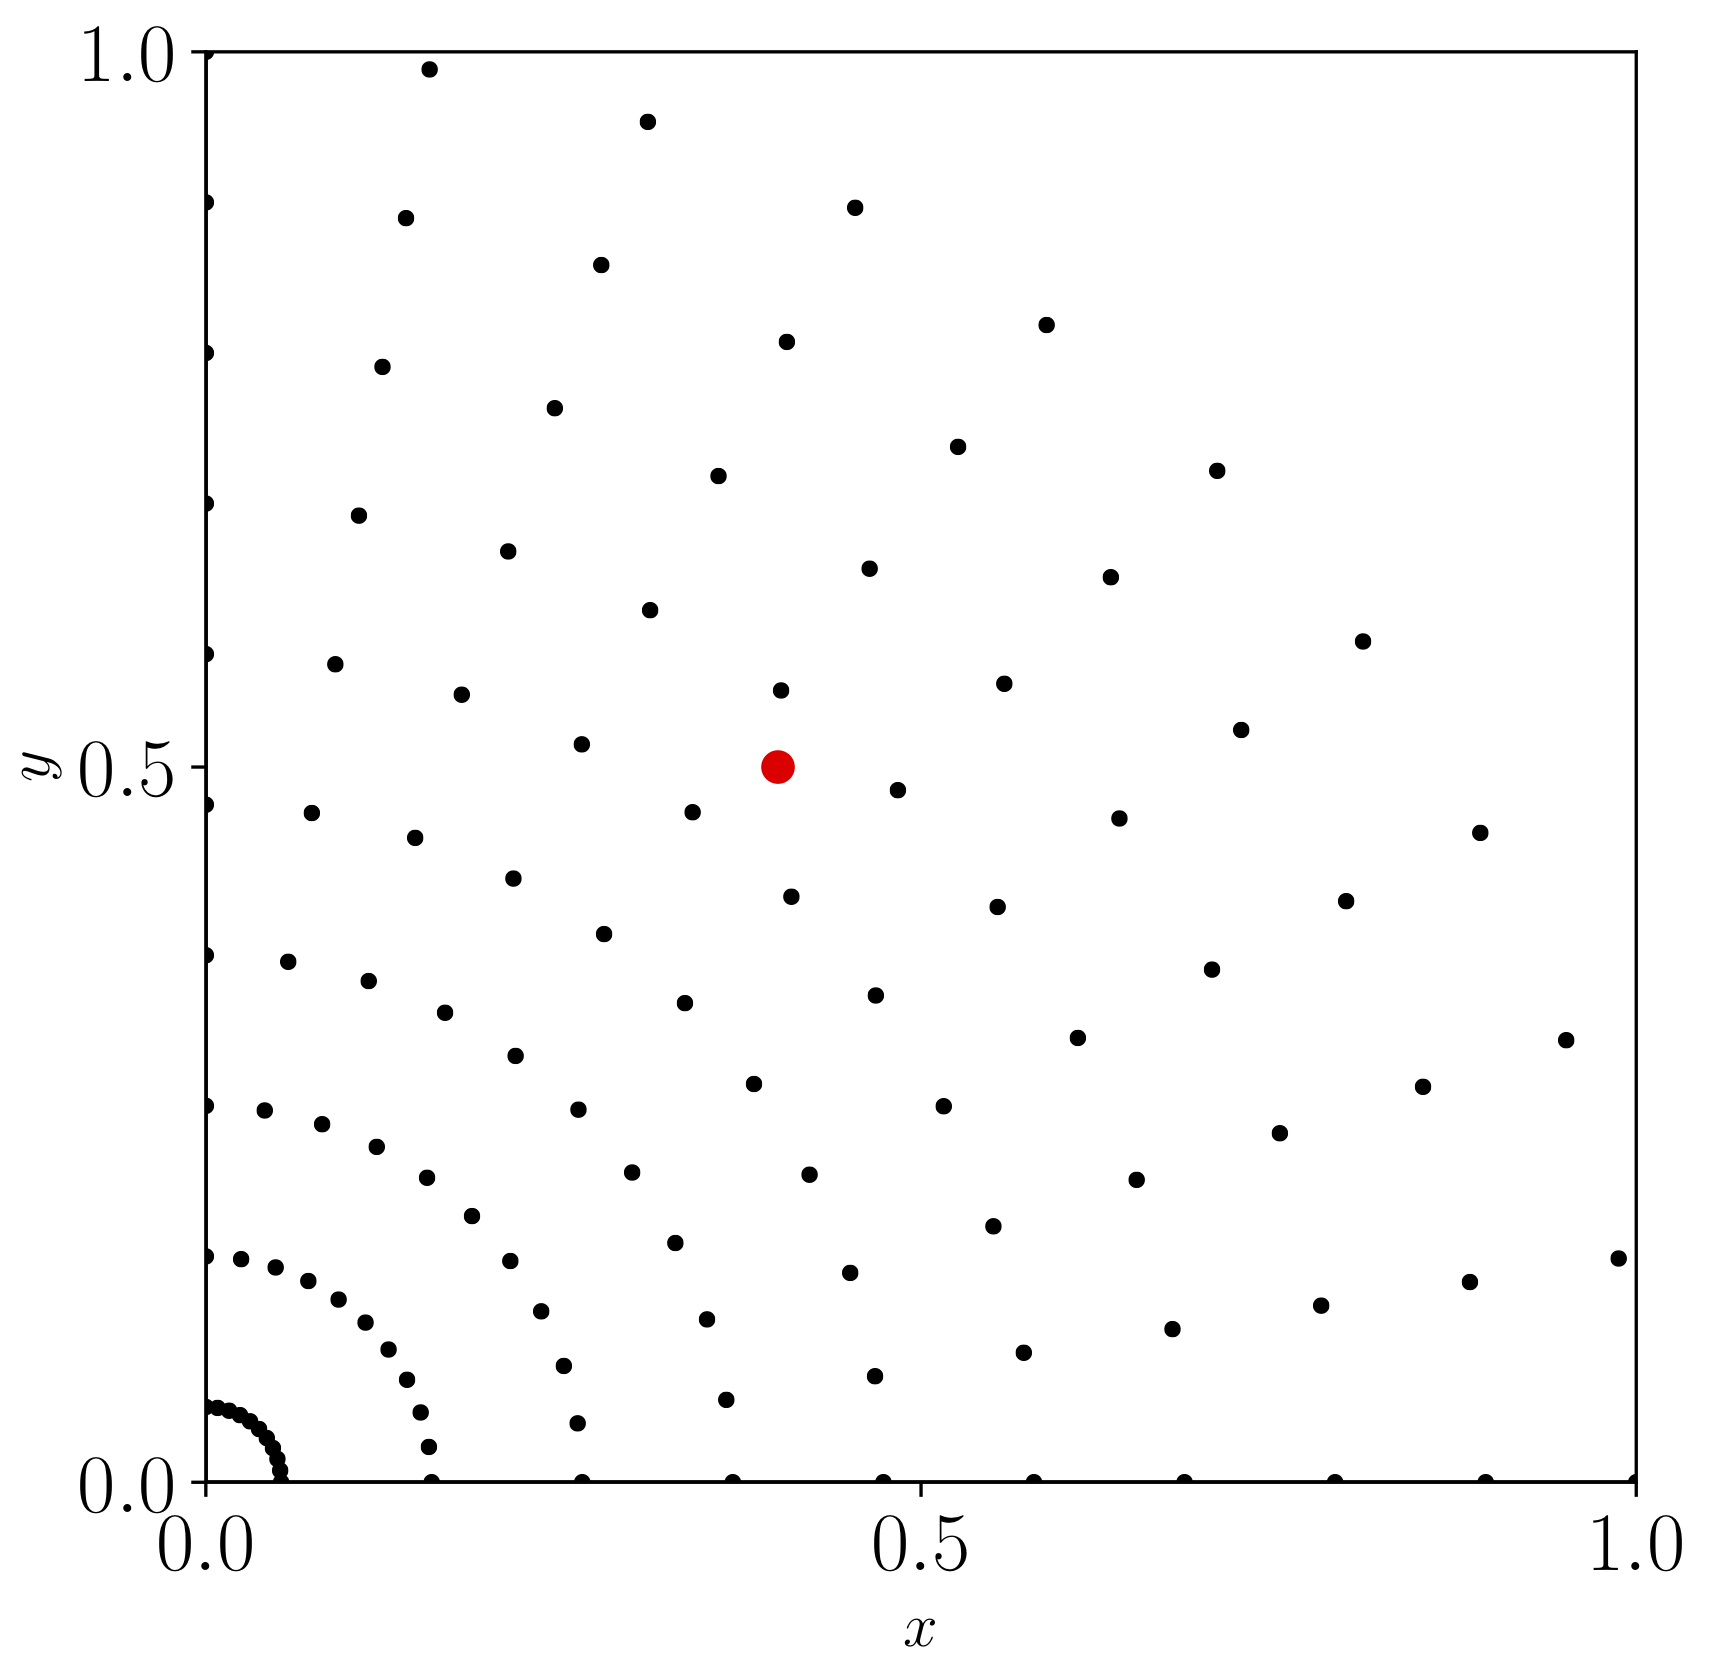
\includegraphics[scale=0.5]{figures/Interp1.png}
	\end{figure}
\end{frame}

\begin{frame}{Interpolation Scheme Example (cont.)}
	\begin{figure}[H]
		\centering
		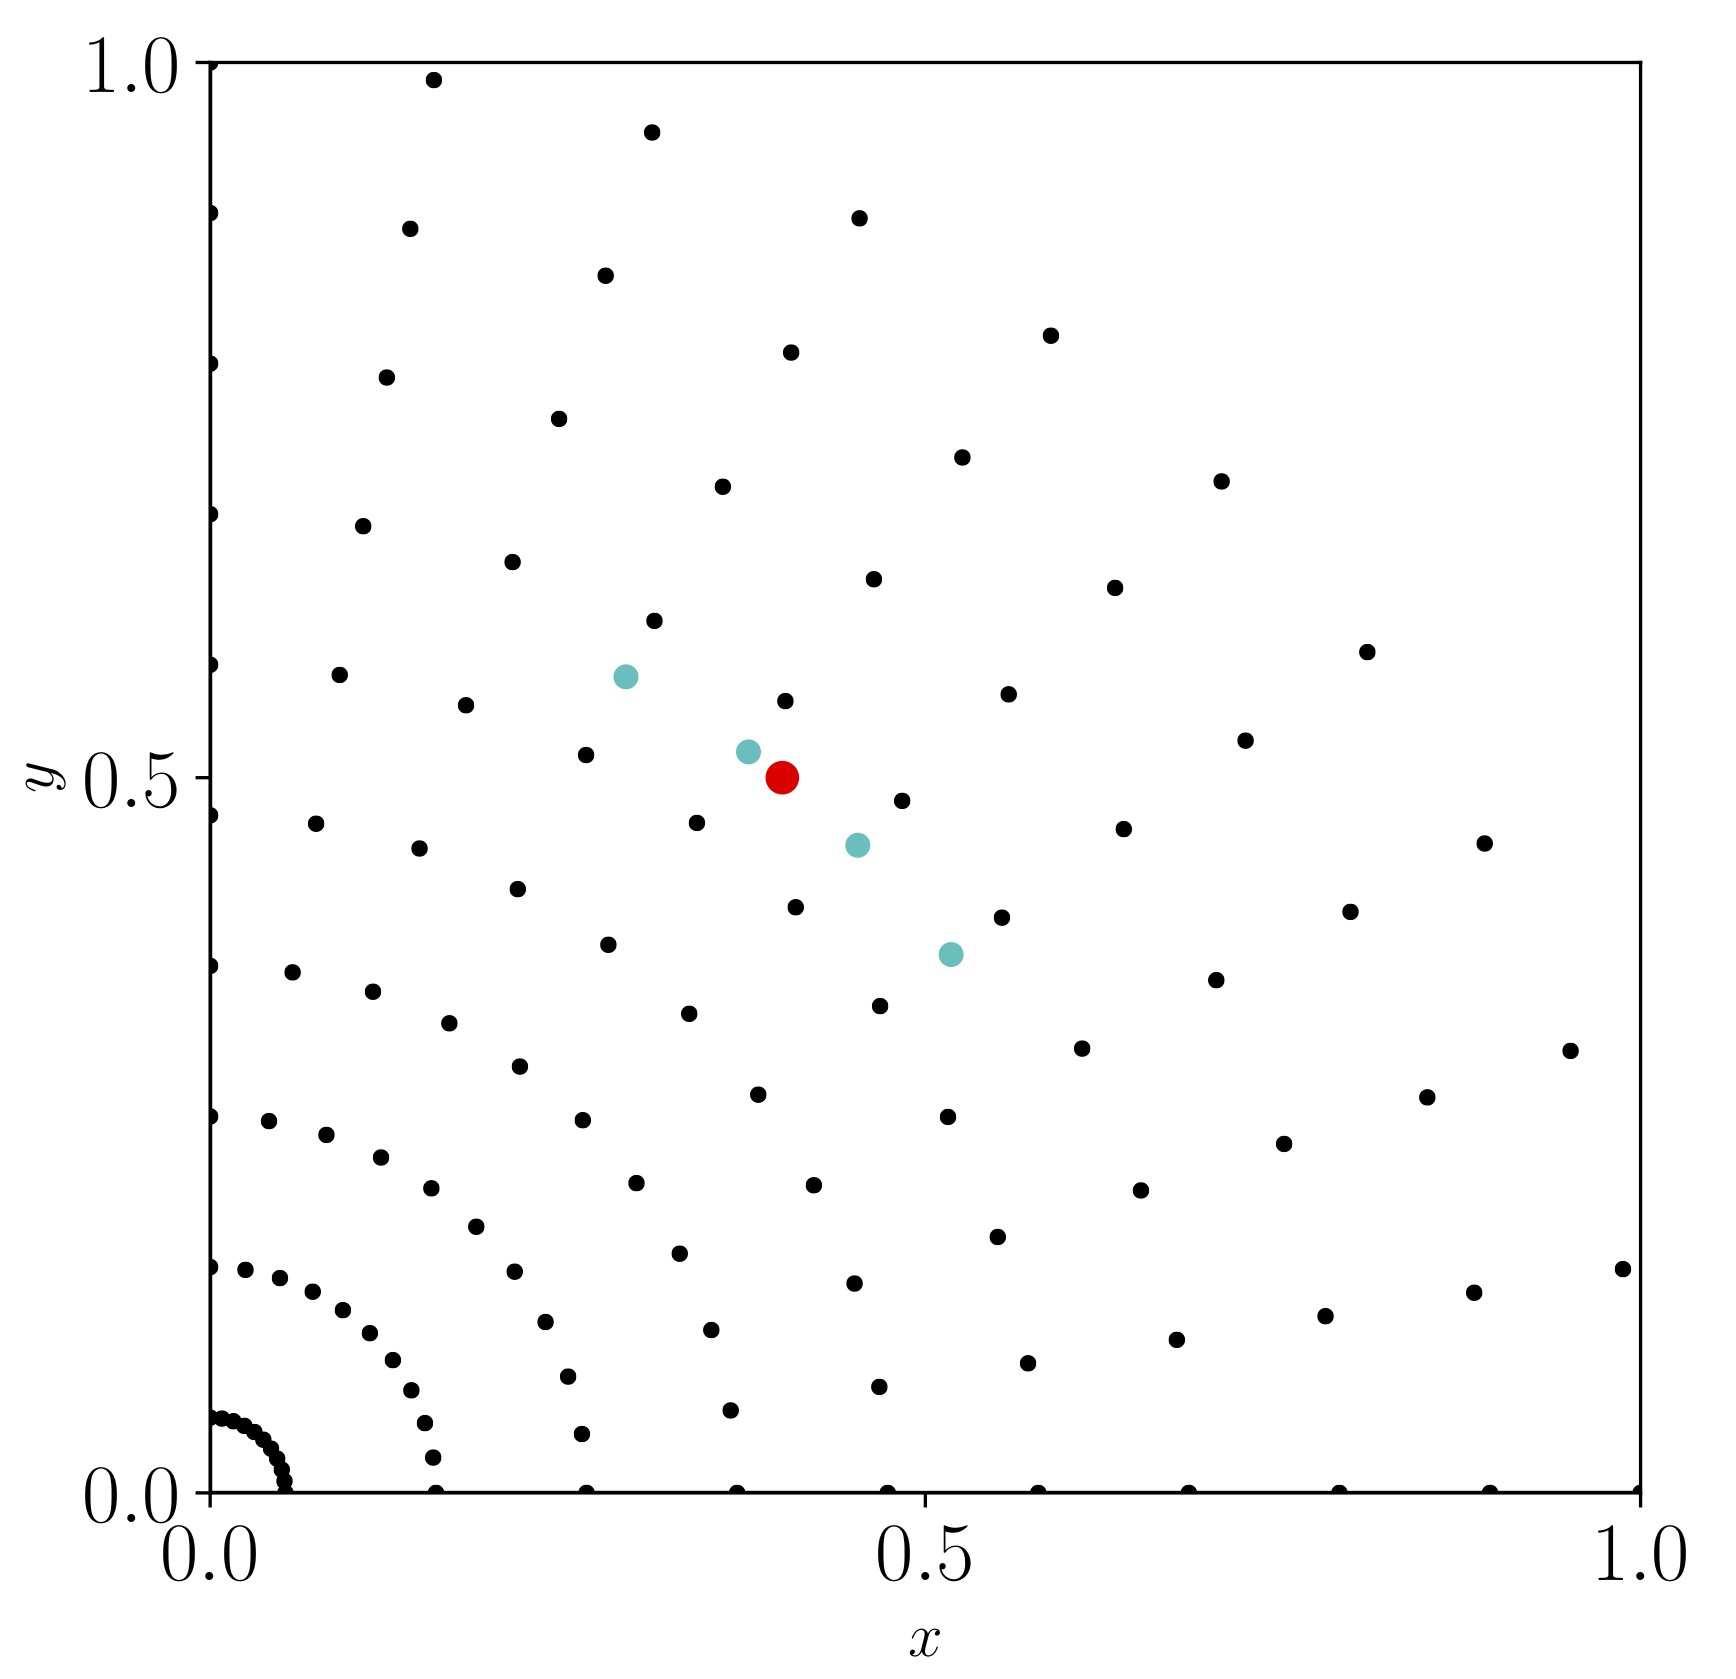
\includegraphics[scale=0.5]{figures/Interp2.png}
	\end{figure}
\end{frame}

\begin{frame}{Interpolation Scheme Example (cont.)}
	\begin{figure}[H]
		\centering
		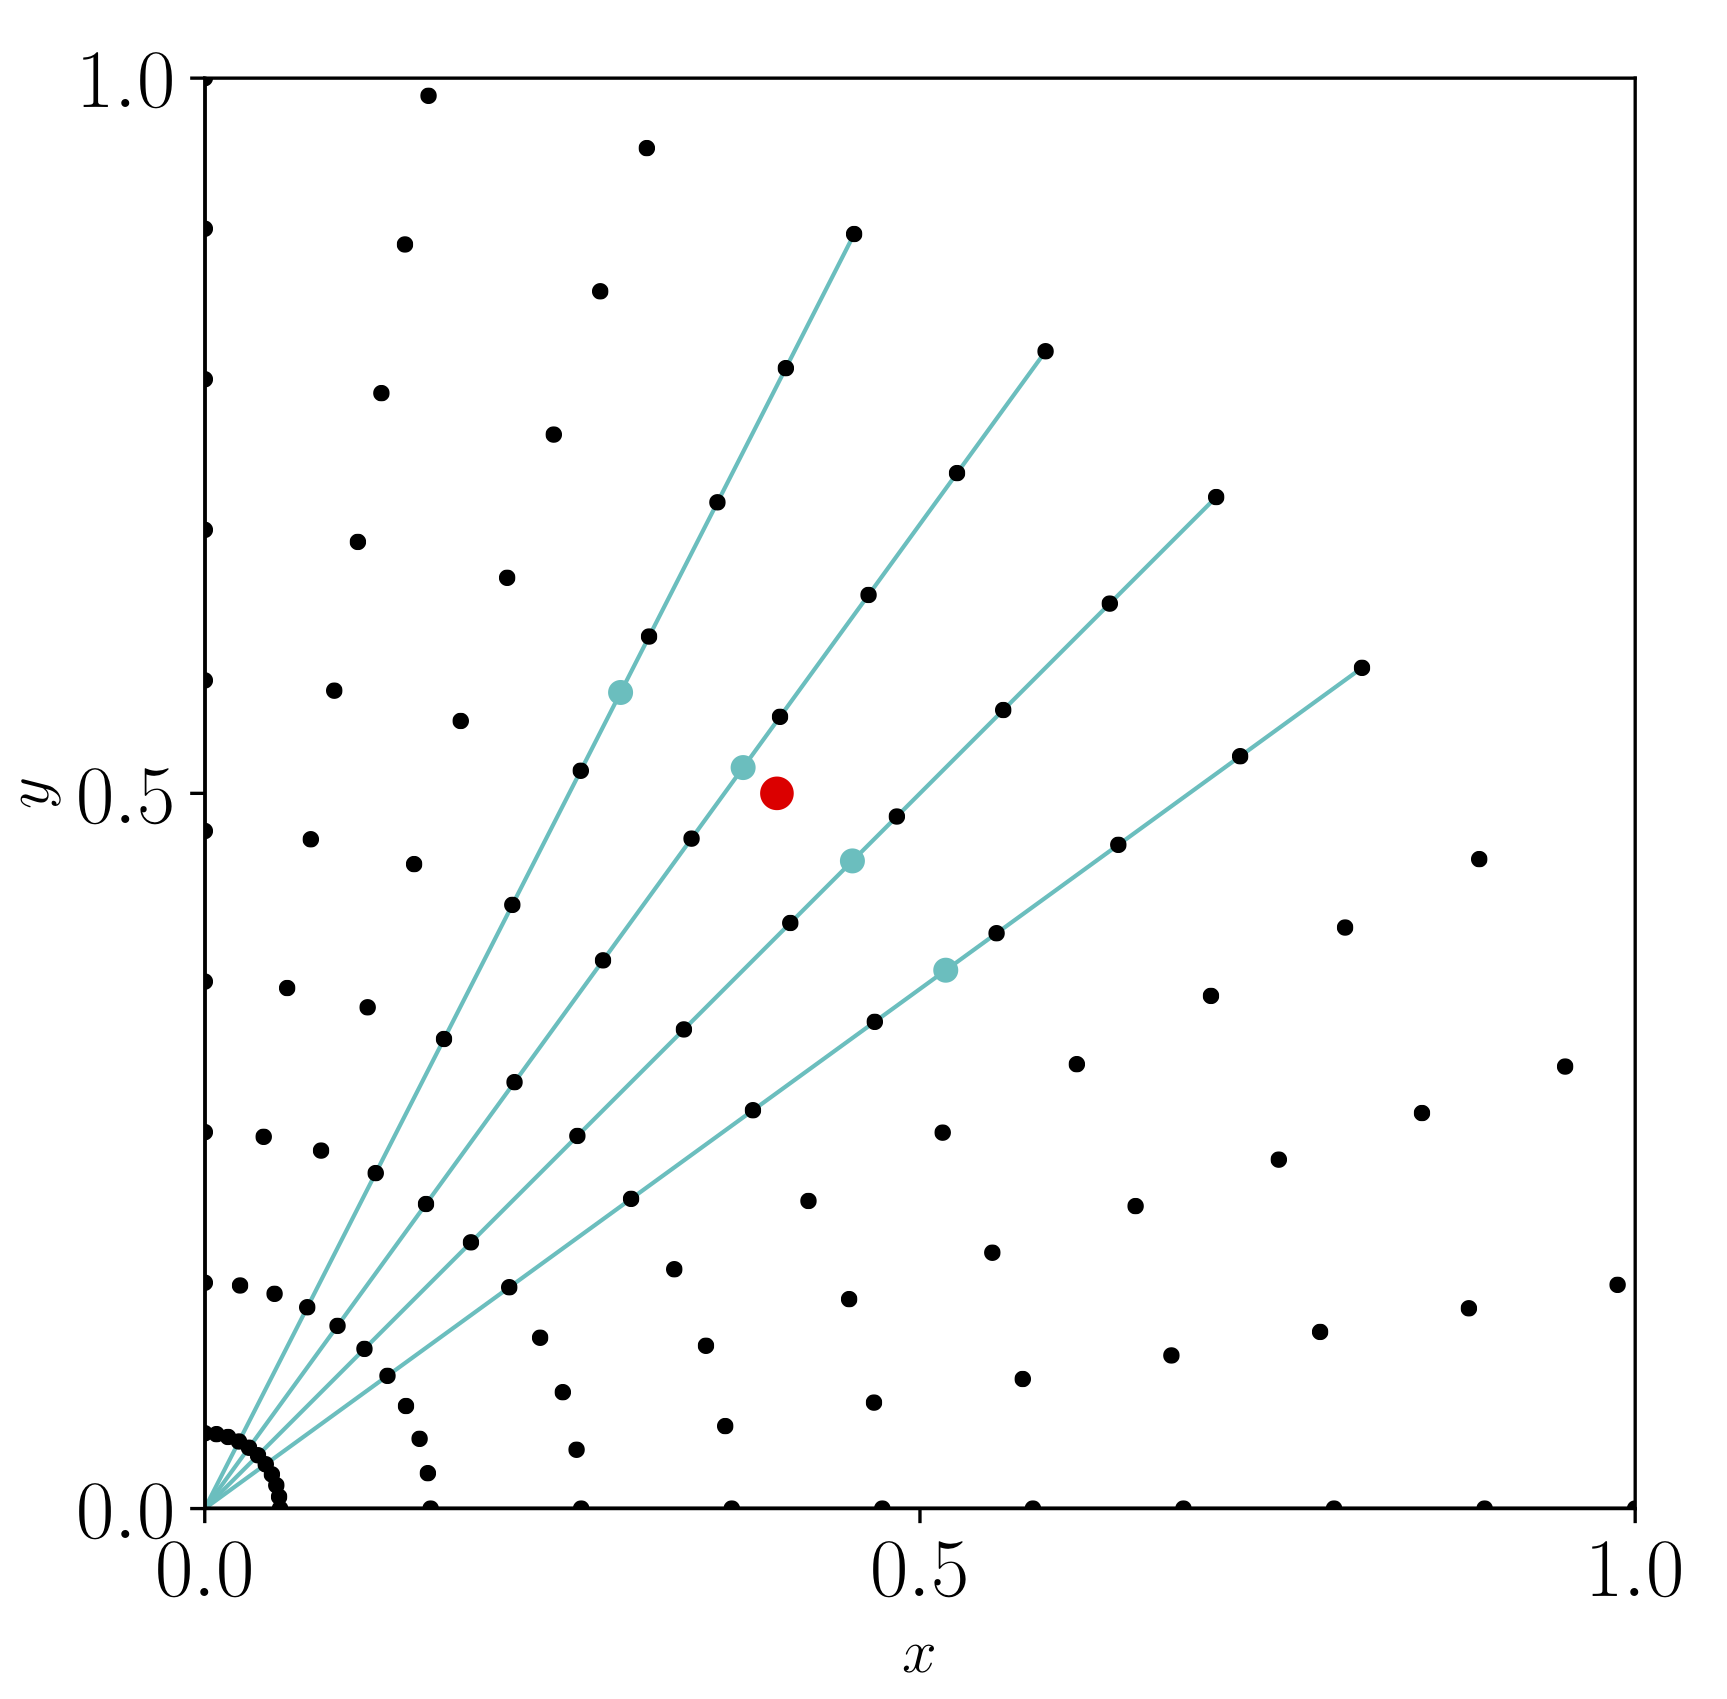
\includegraphics[scale=0.5]{figures/Interp3.png}
	\end{figure}
\end{frame}

\begin{frame}{Interpolation Scheme Example (cont.)}
	\begin{figure}[H]
		\centering
		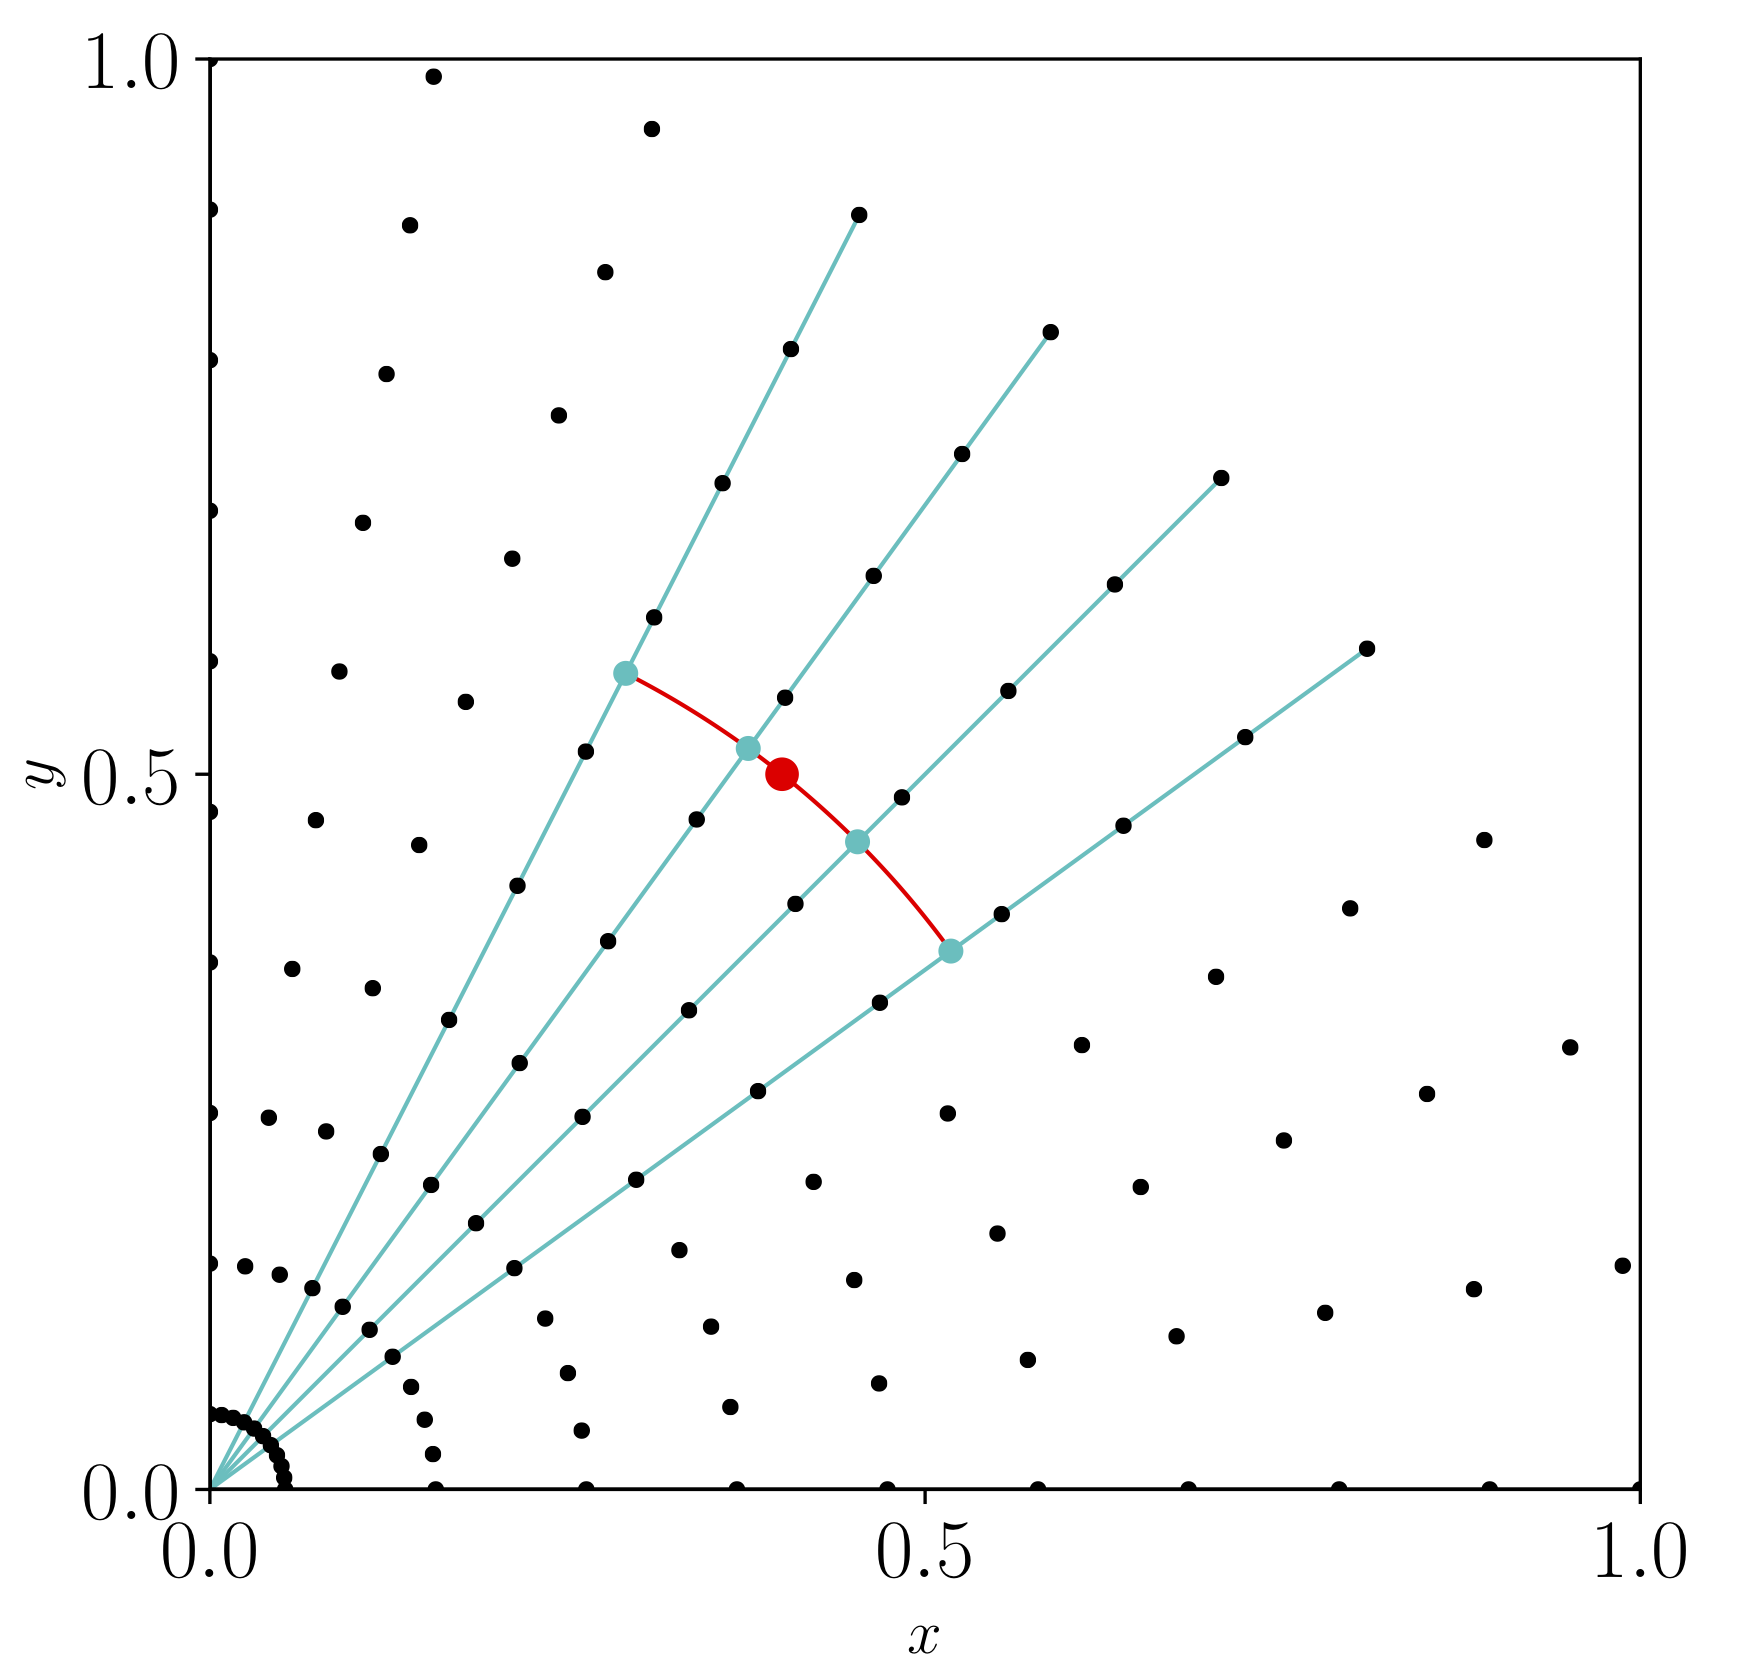
\includegraphics[scale=0.5]{figures/Interp4.png}
	\end{figure}
\end{frame}

\subsection{Computing the Inverse Radon Transform and Backprojection}

% \begin{frame}{Ill-posedness of the IRT}
% 	\begin{itemize}
% 		\item Recall that we have done the following
% 		\begin{itemize}
% 			\item Forward Radon transform multi-dimensional problem
% 			\item Solve systems of one-dimensional advection problems in Radon space to obtain $\widehat{\vec{f_T}}$
% 		\end{itemize}
% 		\item We still have to recover $\vec{f_T}$, the solution at final time in \textit{physical space}
% 		\item This comes down to solving 
% 		\begin{align*}
% 		\mathcal{R} \left(\,\vec{f_T} \right) & = \widehat{\vec{f_T}}
% 		\end{align*}
% 	\end{itemize}
% \end{frame}

\begin{frame}{Ill-posedness of the IRT}
    \begin{itemize}
        \item Suppose $f(x, y): \mathbb{R}^{2} \rightarrow \mathbb{R}$ is a function with compact support, and
        \begin{align*}
            \mathcal{R}(\,f) & = \widehat{f}
        \end{align*}
        \item Is there a way of recovering $f$ given only $\widehat{f}$~?
    \end{itemize}
\end{frame}

\begin{frame}{Ill-posedness of the IRT (cont.)}
	\begin{itemize}
	    \item In discretized case, we only know $f, \, \widehat{f}$ at mesh points
		\item Recall that our mesh is parameterized by two integers
		\begin{itemize}
			\item $N_{\omega}$, the number of angles
			\item $N_{s}$, the number of Chebyshev points along one angle
			\item Total of $N_{\omega} \times N_{s}$ mesh points
		\end{itemize}
		\item Define $\vec{f}, \, \widehat{\vec{f}} \in \mathbb{R}^{N_{\omega} \times N_{s}}$
		such that 
		\begin{align*}
		    \vec{f} & := \text{$f$ evaluated at mesh points} \\
		    \widehat{\vec{f}} & := \text{$\widehat{f}$ evaluated at mesh points}
		\end{align*}
	\end{itemize}
\end{frame}

\begin{frame}{Ill-posedness of the IRT (cont.)}
    \begin{itemize}
        \item Recall we can approximate $\mathcal{R}(\,f)$ with a matrix-vector multiplication
        \item We create a matrix $\mat{R} \in \mathbb{R}^{(N_{s} \times N_{\omega}) \times (N_{s} \times N_{\omega})}$ such that
		\begin{align*}
		    \mat{R} \, \vec{f} & = \widehat{\vec{f}}
		\end{align*}
		where the $j^{th}$ column of $\mat{R}$ is the discretized Radon transform evaluated at $\vec{e_{j}}$
% 		\begin{align*}
% 		    e_{j} & =
% 		    \begin{cases*}
% 		        1 & at $j^{th}$ mesh point \\
% 		        0 & otherwise
% 		    \end{cases*}
% 		\end{align*}
    \end{itemize}
\end{frame}

\begin{frame}{Ill-posedness of the IRT (cont.)}
	\begin{itemize}
		\item The system
		\begin{align*}
		    \mat{R} \, \vec{f} & = \widehat{\vec{f}}
		\end{align*}
		is \textit{very hard} to solve with typical linear algebra techniques
	\end{itemize}
\end{frame}

% \begin{frame}{Approaches to Computing the IRT}
% 	\begin{itemize}
% 		\item For this project, we performed the IRT using two approaches
% 		\begin{itemize}
% 			\item Approximate pseudo-inverse
% 			\begin{itemize}
% 				\item This approach did not pan out
% 			\end{itemize}
% 			\item BiCGSTAB
% 			\begin{itemize}
% 				\item We created a "fake" $\mathcal{R}^T$ that we use as a pre-conditioner for our BiCGSTAB method to find the IRT.
% 			\end{itemize}
% 		\end{itemize}
% 	\end{itemize}
% \end{frame}

\begin{frame}{Approaches to Computing the IRT}
    \begin{itemize}
        \item Note that
        \begin{align*}
            \mat{R} \, \vec{f} = \widehat{\vec{f}} \quad \Longleftrightarrow \quad \mat{R}^{T} \, \mat{R} \, \vec{f} = \mat{R}^{T} \, \widehat{\vec{f}}
        \end{align*}
        \item The system 
        \begin{align*}
            \mat{R}^{T} \, \mat{R} \, \vec{f} = \mat{R}^{T} \, \widehat{\vec{f}}
        \end{align*}
        are the \textbf{normal equations}
        \item What does pre-multiplication by $\mat{R}^{T}$ mean?
    \end{itemize}
\end{frame}

\begin{frame}{Backprojection}
    \begin{itemize}
        \item The adjoint of the Radon transform, denoted $\mathcal{R}^{*}$, is known as \textbf{backprojection}
        \item If $\widehat{f}\left(s, \omega\right): \mathbb{R} \times [0, \pi] \rightarrow \mathbb{R}$, the backprojection of $\widehat{f}$ is
        \begin{align*}
            \mathcal{R}^{*} \left( \widehat{f} \right) (x, y) & := \int_{0}^{\pi} f(x \cos (\omega) + y \sin (\omega), \omega) \, d \omega
        \end{align*}
    \end{itemize}
\end{frame}

\begin{frame}{Graphical Representation of Backprojection}
    \begin{figure}[H]
        \centering
        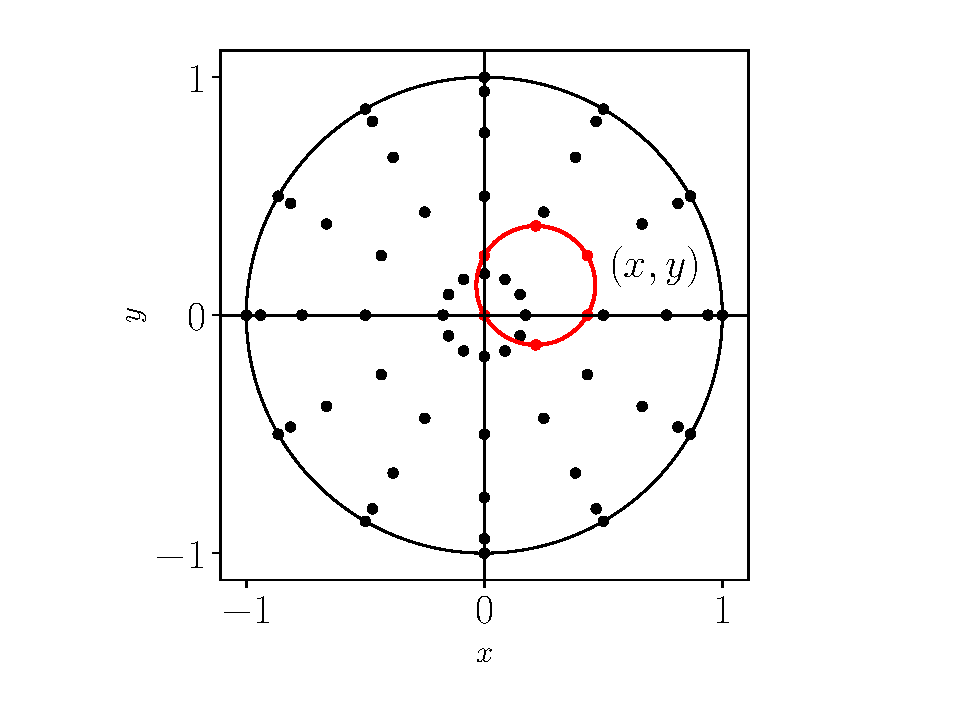
\includegraphics[scale=0.65]{figures/backprojection.pdf}
    \end{figure}
\end{frame}

% \begin{frame}{BiCGSTAB}
% 	\begin{itemize}
% 		\item We created a "fake" $\mathcal{R}^T$ that we use as a pre-conditioner for our BiCGSTAB method to find the IRT.
% 	\end{itemize}
% \end{frame}

\begin{frame}{Backprojection (cont.)}
    \begin{itemize}
        \item We can \textit{approximate} the action of $\mathcal{R}^{*}$ using $\mat{R}^{T}$
        \item Recall we want to solve
        \begin{align*}
            \mat{R}^{T} \, \mat{R} \, \vec{f} & = \mat{R}^{T} \, \widehat{\vec{f}}
        \end{align*}
        \item However, $\mat{R}$  is \textit{very} large in practice
        \begin{itemize}
            \item $N_{s}$ and $N_{\omega}$ dictate how well we can recover $\vec{f}$
        \end{itemize}
    \end{itemize}
\end{frame}

\begin{frame}{Using BiCGSTAB to Solve the Normal Equations}
    \begin{itemize}
        \item We do not explicitly need $\mat{R}^{T} \, \mat{R}$, just the matrix-vector products $\mat{R} \, \vec{f}$, $\mat{R}^{T} \left(\mat{R} \, \, \vec{f} \right)$
        \item We use an iterative method (BiCGSTAB) to solve
        \begin{align*}
            \mat{R}^{T} \, \mat{R} \, \vec{f} & = \mat{R}^{T} \, \widehat{\vec{f}}
        \end{align*}
        by minimizing successive residuals
        \begin{align*}
            \left\| \mat{R}^{T} \, \widehat{\vec{f}} - \mat{R}^{T} \, \mat{R} \, \vec{f}^{(k)} \right\|_{2}
        \end{align*}
        over $\text{span} \{ \vec{r_0}, \left( \mat{R}^{T} \, \mat{R} \right) \, \vec{r_0}, \hdots, \}$ where $\vec{r_0} = \mat{R}^{T} \, \mat{R} \vec{f}^{(0)} - \mat{R}^{T} \, \vec{\widehat{f}}$
    \end{itemize}
\end{frame}

% \begin{frame}{Ill-posedness of the IRT (cont).}
% \begin{itemize}
%     \item
%         Radon transform is near-singular, inverse difficult to compute exactly 
%     \begin{itemize}
%         \item
%             $\mathcal{R}\left(\,\vec{f}\right) = \widehat{\vec{f}}$ can be solved with BICGSTAB, but is expensive
%     \end{itemize}
%     \item
%         For a given grid of points, construct an invertible matrix such that $\mat{R} \, \vec{f} = \widehat{\vec{f}}$ and $\mat{R}^{-1} \, \widehat{\vec{f}} = \vec{f}$
%     \begin{itemize}
%         \item
%             Consider $e_i$, the $i$-th basis vector of $\mathbb{R}^{Ns \times N\omega}$
%         \item
%             Computing $\mathcal{R}(e_i)$ produces the $i$-th column of $\mat{R}$
%     \end{itemize}
% \end{itemize}
% \end{frame}

%\subsection*{Wide matrix}

% \begin{frame}{Wide Matrix}
% \begin{itemize}
%     \item
%         An issue that we came across when working with the IRT was that  $\widehat{f}$ was not in the the range of $\mathcal{R}$. %Radon matrix
%     \item
%         A possible solution that we came up with would be to increase the size of $\mathcal{R}$ in the $\omega$ direction so that the range of $\mathcal{R}$ was larger.
% \end{itemize}
% \end{frame}

\section{Hyperbolic PDEs}
\subsection{The Radiative Transfer Problem}


\begin{frame}{Application: Radiative Transfer}
	\begin{itemize}
		\item 
			We want to solve the \textbf{Radiative Transfer Equation}
		\begin{align*}
			F_{,t} + \vec{\Omega} \cdot \vec{\nabla}F + \sigma_t F = \frac{\sigma_s}{4\pi}\int_{\mathbb{S}^2}F\, d\vec{\Omega}
		\end{align*}
		\item
			A kinetic model for subatomic particles propagating through a homogeneous medium
		\begin{itemize}
			\item $\vec{\Omega} \cdot \vec{\nabla}F$ is a transport term
			\item $ \frac{\sigma_s}{4\pi}\int_{\mathbb{S}^2}F\, d\vec{\Omega} - \sigma_t\,F$ is a collision term
		\end{itemize}
		\item
			$F(t, \vec{x}, \vec{\Omega}) : \mathbb{R}^+ \times \mathbb{R}^3 \times \mathbb{S}^2 \to \mathbb{R}$ is the distribution function for particles at a specific location and with a specific velocity
		\item
			A linear transport equation in $1 + 5$ dimensions
	\end{itemize}
\end{frame}

\begin{frame}{Spherical Harmonics}
	\begin{itemize}
		\item
			Use spherical harmonics to create $P_N$ equations
		\begin{align*}
		F(t, \vec{x}, \vec{\Omega}) \approx \sum_{\ell = 0}^N \sum_{m=-\ell}^\ell F_\ell^m(t, \vec{x})Y_\ell^m(\mu, \phi)
		\end{align*}	
		\item 
			Already know spherical harmonics, $Y_\ell^m(\mu, \phi)$; removes angular dependence from $F$
		\item
			Need to solve for (most) of the $F_\ell^m(t, \vec{x})$
	\end{itemize}
\end{frame}
\begin{frame}{$P_N$ Equations}
	\begin{itemize}
		\item
		For a given positive, odd $N$, the $P_N$ approximation yields a system of $\frac{1}{2}(N+1)(N+2)$ linear differential equations
		\item
		For $P_1$ in 2D, the equations are
		\begin{align*}
		F_{0,t}^0 - \sqrt{\frac{2}{3}}\,F_{1,x}^1 + \sqrt{\frac{1}{3}}\,F_{1,y}^0 & = -\sigma_a\,F_0^0 \\
		F_{1,t}^0 + \sqrt{\frac{1}{3}}\,F_{0,y}^0 & = -(\sigma_a + \sigma_s)\,F_1^0 \\
		F_{1,t}^1 - \sqrt{\frac{1}{6}}\,F_{0,y}^0 & = -(\sigma_a + \sigma_s)\,F_1^1
		\end{align*}
		for unknown functions $F_0^0(x, y)$, $F_1^0(x, y)$, and $F_1^1(x, y)$
	\end{itemize}
\end{frame}

\begin{frame}{$P_N$ Equation Matrices}
	\begin{itemize}
		\item
		Can be written as $\vec{F}_{,t} + \mat{A}\, \vec{F}_{,x} + \mat{B} \, \vec{F}_{,y} = \mat{C} \, \vec{F}$ with the following matrices:
	\end{itemize}
	\begin{align*}
	\vec{F} = 
	\begin{bmatrix}
	F_0^0 \\
	F_1^0 \\
	F_1^1
	\end{bmatrix} \quad
	&\mat{A} = 
	\begin{bmatrix}
	0 & 0 & -\sqrt{\frac{2}{3}} \\
	0 & 0 & 0 \\
	-\sqrt{\frac{1}{6}} & 0 & 0
	\end{bmatrix} \\
	\mat{B} = 
	\begin{bmatrix}
	0 & \sqrt{\frac{1}{3}} & 0 \\
	\sqrt{\frac{1}{3}} & 0 & 0 \\
	0 & 0 & 0
	\end{bmatrix} \quad
	&\mat{C} = 
	\begin{bmatrix}
	-\sigma_a & 0 & 0 \\
	0 & -(\sigma_a + \sigma_s) & 0 \\
	0 & 0 & -(\sigma_a + \sigma_s)
	\end{bmatrix}
	\end{align*}
\end{frame}

\subsection{Radon Transforms of Derivatives}
\begin{frame}{Solving the $P_N$ Equations}
	\begin{itemize}
		\item
		We now consider the following system of $M$ differential equations
		\begin{align*}
		\vec{q}_{,t} + \mat{A}\,\vec{q}_{,x} + \mat{B}\,\vec{q}_{,y} & = \mat{C}\,\vec{q} \\
		\vec{q}(t = 0, x, y) & = \vec{q}_{0}(x, y)
		\end{align*}
		where
		\begin{itemize}
			\item $q(t, x, y): \mathbb{R}_{\geq 0} \times \mathbb{R}^{2} \rightarrow \mathbb{R}^{M}$ is a vector valued function
			\item $\mat{A}, \mat{B}, \mat{C} \in \mathbb{R}^{M \times M}$
		\end{itemize}
		\vspace{0.5cm}
		\item \textbf{Claim:} the Radon transform simplifies spatial derivatives
	\end{itemize}   
\end{frame}

% \begin{frame}{Radon Transform of the PDE}
% 	\begin{itemize}
% 		\item Recall the definition of the Radon transform, where $z$ is the axis perpendicular to $s$ after a rotation by $\omega$:
% 		\begin{align*}
% 			\mathcal{R}(f(x, y)) = \widehat{f}(s, \omega) = \int_{-\infty}^{\infty} f(\,x, y\,) \, dz
% 		\end{align*}
% 		% \item Using the linearity of $\mathcal{R}$, apply it to each term of the PDE
% 		\item Apply $\mathcal{R}$ to the PDE and use linearity of the operator
% 		\begin{align*}
% 			&\mathcal{R}{\left( \vec{q}_{,t} + \mat{A}\, \vec{q}_{,x} + \mat{B} \, \vec{q}_{,y} = \mat{C} \, \vec{q} \right)} \\
% 			\implies & \mathcal{R}{\left( \vec{q}_{,t} \right)} + \mat{A} \,\mathcal{R}{\left(  \vec{q}_{, x} \right)} + \mat{B} \,\mathcal{R}{\left(  \vec{q}_{, y} \right)} = \mat{C} \, \mathcal{R}{\left(  \vec{q} \right)}
% 		\end{align*}
% 		\item Note: $\mathcal{R}\left(\vec{f}\right)$ means applying $\mathcal{R}$ to each element of $\vec{f}$
% 	\end{itemize}
% \end{frame}

\begin{frame}{Radon Transform of the PDE}
	\begin{itemize}
		% \item Using the linearity of $\mathcal{R}$, apply it to each term of the PDE
		\item Apply $\mathcal{R}$ to the PDE at an angle $\omega$
		\begin{align*}
			\onslide<1->{& \mathcal{R}{\left( \vec{q}_{,t} + \mat{A}\, \vec{q}_{,x} + \mat{B} \, \vec{q}_{,y} = \mat{C} \, \vec{q} \right)} \\}
			\onslide<2->{\implies & \mathcal{R}{\left( \vec{q}_{,t} \right)} + \mat{A} \,\mathcal{R}{\left(  \vec{q}_{, x} \right)} + \mat{B} \,\mathcal{R}{\left(  \vec{q}_{, y} \right)} = \mat{C} \, \mathcal{R}{\left( \vec{q} \right)}}
		\end{align*}
		\only<2->{\item \textbf{Note:} $\mathcal{R}\left(\,\vec{f}\right)$ means applying $\mathcal{R}$ to each element of $\vec{f}$}
	\end{itemize}
\end{frame}

\begin{frame}{Radon Transforms of Partial Derivatives}
	\begin{itemize}
		\item By the chain rule,
		\begin{align*}
		\frac{\partial}{\partial x} & = \frac{\partial s}{\partial x} \frac{\partial}{\partial s} + \frac{\partial z}{\partial x} \frac{\partial}{\partial z} \\
		\frac{\partial}{\partial y} & = \frac{\partial s}{\partial y} \frac{\partial}{\partial s} + \frac{\partial z}{\partial y} \frac{\partial}{\partial z}
		\end{align*}
		%\pause 
		\item
		From our earlier definitions of $s$ and $z$, we obtain
		\begin{align*}
		    \frac{\partial}{\partial x} & = \cos (\omega) \frac{\partial}{\partial s} -\sin (\omega) \frac{\partial}{\partial z} \\
		    \frac{\partial}{\partial y} & = \sin (\omega) \frac{\partial}{\partial s} + \cos (\omega) \frac{\partial}{\partial z}
		\end{align*}
		
		% \begin{align*}
		% \frac{\partial s}{\partial x} & = \cos (\omega) & \frac{\partial s}{\partial y} & = \sin (\omega) \\
		% \frac{\partial z}{\partial x} & = -\sin (\omega) & \frac{\partial z}{\partial y} & = \cos (\omega)
		% \end{align*}
	\end{itemize}
\end{frame}

% \begin{frame}{Radon Transforms of Derivatives}
% 	\begin{itemize}
% 		\item
% 		We can now compute $\mathcal{R}\left(\,f_{,x}\right)$
% 		\begin{align*}
%     		\mathcal{R}\left(\,f_{,x}\right) & = \int_{-\infty}^{\infty} f_{, x} \, dz  \\
%     		& = \int_{-\infty}^{\infty}  \left( \cos (\omega) \, f_{, s} - \sin (\omega) \, f_{, z} \right) \, dz \\
%     		& = \cos (\omega) \int_{-\infty}^{\infty} f_{, s} \, dz - \sin (\omega) \int_{-\infty}^{\infty} f_{, z} \, dz \\
%     		& = \cos (\omega) \frac{\partial}{\partial s} \int_{-\infty}^{\infty} f\,dz - \sin (\omega) \left[\, f(z = +\infty) - f(z = -\infty) \right] \\
%     		& = \cos (\omega) \, \frac{\partial}{\partial s} \mathcal{R}(f) \\
%     		& = \cos (\omega) \, \widehat{f}_{,s}
% 		\end{align*}
% 	\end{itemize}
% \end{frame}

\begin{frame}{Radon Transform of Partial Derivatives}
    \begin{itemize}
        \item Recall the definition of the Radon transform, where $z$ is the axis perpendicular to $s$ after a rotation by $\omega$:
		\begin{align*}
			\mathcal{R}(\,f(x, y)) = \widehat{f}(s, \omega) = \int_{-\infty}^{\infty} f(\,x, y\,) \, dz
		\end{align*}
    \end{itemize}    
\end{frame}

\begin{frame}{Radon Transforms of Partial Derivatives}
	\begin{itemize}
		\item
		We can now compute $\mathcal{R}\left(\,f_{,x}\right)$
		\begin{align*}
    		\onslide<1->{\mathcal{R}\left(\,f_{,x}\right) & = \int_{-\infty}^{\infty} f_{, x} \, dz  \\}
    		\onslide<2->{& = \int_{-\infty}^{\infty}  \left( \cos (\omega) \, f_{, s} - \sin (\omega) \, f_{, z} \right) \, dz \\}
    		\onslide<3->{& = \cos (\omega) \int_{-\infty}^{\infty} f_{, s} \, dz - \sin (\omega) \int_{-\infty}^{\infty} f_{, z} \, dz \\}
    		\onslide<4->{& = \cos (\omega) \frac{\partial}{\partial s} \int_{-\infty}^{\infty} f\,dz - \sin (\omega) \left[\, f(z = +\infty) - f(z = -\infty) \right] \\}
    		\onslide<5->{& = \cos (\omega) \, \frac{\partial}{\partial s} \mathcal{R}(\,f) \\}
    		\onslide<6->{& = \cos (\omega) \, \widehat{f}_{,s}}
		\end{align*}
	\end{itemize}
\end{frame}

\begin{frame}{Radon Transforms of Partial Derivatives}
	\begin{itemize}
		\item
		$\mathcal{R}\left(\,f_{,y}\right)$ can be computed similarly
		\begin{align*}
    		\mathcal{R}\left(\,f_{,y}\right) & = \int_{-\infty}^{\infty} f_{, y} \, dz  \\
    		& = \int_{-\infty}^{\infty}  \left( \sin (\omega) \, f_{, s} - \cos (\omega) \, f_{, z} \right) \, dz \\
    		& = \sin (\omega) \int_{-\infty}^{\infty} f_{, s} \, dz - \cos (\omega) \int_{-\infty}^{\infty} f_{, z} \, dz \\
    		& = \sin (\omega) \frac{\partial}{\partial s} \int_{-\infty}^{\infty} f\,dz - \cos (\omega) \left[\, f(z = +\infty) - f(z = -\infty) \right] \\
    		& = \sin (\omega) \, \frac{\partial}{\partial s} \mathcal{R}(\,f) \\
    		& = \sin (\omega) \, \widehat{f}_{,s}
		\end{align*}
	\end{itemize}
\end{frame}

\begin{frame}{Radon Transforms of Partial Derivatives}
	\begin{itemize}
		\item The Radon transform is a spatial transformation, thus:
		\begin{align*}
			\mathcal{R}\left(\,f_{,t}\right) = \frac{\partial}{\partial t}\mathcal{R}(\,f) = \widehat{f}_{,t}
		\end{align*}
		\item In summary, 
		\begin{align*}
    		\mathcal{R}(\,f_{, t}) & = \widehat{f}_{, t} \\ % \frac{\partial}{\partial t} \, \mathcal{R}(f) \\
    		\mathcal{R}(\,f_{, x}) & = \cos (\omega) \, \widehat{f}_{, s} \\ % \frac{\partial}{\partial s} \, \mathcal{R}(f) \\
    		\mathcal{R}(\,f_{, y}) & = \sin (\omega) \, \widehat{f}_{, s}  % \frac{\partial}{\partial s} \, \mathcal{R}(f)
		\end{align*}
		\item
			All spatial derivatives in $xy$ space become derivatives of $s$
	\end{itemize}
\end{frame}

\begin{frame}{Radon Transform of the PDE}
	\begin{itemize}
		\item Can now complete the transformation and add like terms:
		\begin{align*}
		    \onslide<1->{& \mathcal{R}{\left( \vec{q}_{,t} + \mat{A}\, \vec{q}_{,x} + \mat{B} \, \vec{q}_{,y} = \mat{C} \, \vec{q} \right)} \\ \\}
			\onslide<2->{\implies & \mathcal{R}{\left( \vec{q}_{,t} \right)} + \mat{A} \,\mathcal{R}{\left(  \vec{q}_{, x} \right)} + \mat{B} \,\mathcal{R}{\left(  \vec{q}_{, y} \right)} = \mat{C} \, \mathcal{R}{\left(  \vec{q} \right)} \\ \\}
			\onslide<3->{\implies & \widehat{\vec{q}}_{, t} + \cos (\omega) \, \mat{A} \, \widehat{\vec{q}}_{, s} + \sin (\omega) \, \mat{B} \, \widehat{\vec{q}}_{, s} = \mat{C} \, \widehat{\vec{q}} \\ \\}
			\onslide<4->{\implies & \vec{\widehat{q}}_{,t} + \left( \cos (\omega) \, \mat{A} + \sin (\omega) \, \mat{B} \, \right)\vec{\widehat{q}}_{,s} = \mat{C}\,\vec{\widehat{q}}}
		\end{align*}
	\end{itemize}
\end{frame}

\begin{frame}{Radon Transform of the PDE}
	\begin{itemize}
		\item Given 
		\begin{align*}
			\vec{\widehat{q}}_{,t} + \left( \cos (\omega) \, \mat{A} + \sin (\omega) \, \mat{B} \, \right)\vec{\widehat{q}}_{,s} = \mat{C}\,\vec{\widehat{q}}
		\end{align*}
		let $\widetilde{\mat{A}}(\omega) :=  \cos (\omega) \, \mat{A} + \sin (\omega) \, \mat{B}\,$ so that
		\begin{align*}
		\vec{\widehat{q}}_{,t} + \widetilde{\mat{A}}(\omega) \vec{\widehat{q}}_{,s} & = \mat{C}\,\vec{\widehat{q}} \\
		\widehat{\vec{q}}(t = 0, s, \omega) & = \widehat{\vec{q}}_{0}(s, \omega)
		\end{align*}
		\item For each $\omega$, we now have a system of one dimensional PDEs which can be solved with traditional methods
	\end{itemize}
\end{frame}

\begin{frame}{Radon Transform of the PDE}
    \begin{itemize}
        \item To recap: we transformed the 2D system of PDEs
        \begin{align*}
            \vec{q}_{, t} + \mat{A} \, \vec{q}_{, x} + \mat{B} \, \vec{q}_{, y} & = \mat{C} \, \vec{q} \\
                                                                  \vec{q}(t = 0, x, y) & = \vec{q_{0}}(x, y)
        \end{align*}
        into a collection of 1D systems of PDEs
        \begin{align*}
            \widehat{\vec{q}}_{,t} + \widetilde{\mat{A}} (\omega) \, \widehat{\vec{q}}_{,s} & = \mat{C} \, \widehat{\vec{q}} \\
                                                        \widehat{\vec{q}}(t = 0, s, \omega) & = \widehat{\vec{q_{0}}}(s, \omega)
        \end{align*}
        that we can now solve, angle by angle
    \end{itemize}

\end{frame}

\begin{frame}{Defining Hyperbolicity}
	
    \begin{itemize}
    	\item We say the PDE $\, \vec{q}_{, t} + \mat{A} \, \vec{q}_{, x} + \mat{B} \, \vec{q}_{, y} = \mat{C} \, \vec{q} \,$ is \textbf{hyperbolic} if
    	\begin{align*}
    	\widetilde{\mat{A}}(\alpha) := \cos (\alpha) \, \mat{A} + \sin (\alpha) \, \mat{B}
    	\end{align*}
    	is diagonalizable with only real eigenvalues for all $\alpha \in \mathbb{R}$
    	\item Physically, this means that information in the system travels at a finite speed
	    % \item The heat equation is \textit{not} hyperbolic
    	% \item The wave equation is hyperbolic
	    % \item The $P_N$ equations are also hyperbolic
	    \item The wave equation and $P_N$ equations are hyperbolic

    \end{itemize}
\end{frame}
\subsection{Discretization of the PDE}

\begin{frame}{Decoupling the System}
    \begin{itemize}
    	\item After transforming, our $P_N$ formulation is of the form
   		\begin{align*}
    		&\vec{\widehat{q}}_{,t} + \left( \cos (\omega) \, \mat{A} + \sin (\omega) \, \mat{B} \, \right) \vec{\widehat{q}}_{,s} = \mat{C}\,\vec{\widehat{q}} \\
    		&\vec{\widehat{q}}_{,t} + \widetilde{\mat{A}}(\omega) \vec{\widehat{q}}_{,s} = \mat{C}\,\vec{\widehat{q}}
    	\end{align*}
    	\item 
	    	Recall that $\widetilde{\mat{A}} (\omega)$ is diagonalizable with only real eigenvalues for all $\omega \in \mathbb{R}$
        \item We can then write
        \begin{align*}
            \widetilde{\mat{A}}(\omega) & = \mat{P} \, \mat{\Lambda} \, \mat{P}^{-1}
        \end{align*}
        where $\mat{\Lambda}$ is a diagonal matrix of the eigenvalues of $\widetilde{\mat{A}}(\omega)$
    \end{itemize}
\end{frame}

\begin{frame}{Decoupling the System}
    \begin{itemize}
        \item Rewrite system using eigendecomposition of $\widetilde{\mat{A}}(\omega)$
        \begin{align*}
            \onslide<1->{ \widehat{\vec{q}}_{,t} & + \widetilde{\mat{A}}(\omega) \, \widehat{\vec{q}}_{,s} = \mat{C} \, \widehat{\vec{q}} \\}
            \onslide<2->{\Rightarrow \,  \widehat{\vec{q}}_{,t} & + \mat{P} \, \mat{\Lambda} \, \mat{P}^{-1} \, \widehat{\vec{q}}_{,s} = \mat{C} \, \widehat{\vec{q}} \\} 
            \onslide<3->{\Rightarrow  \mat{P}^{-1} \,  \widehat{\vec{q}}_{,t} & + \mat{\Lambda} \, \mat{P}^{-1} \, \widehat{\vec{q}}_{,s} = \mat{P}^{-1} \, \mat{C} \, \widehat{\vec{q}} \\}
            \onslide<4->{\Rightarrow  \frac{\partial}{\partial t}  \left(\, \mat{P}^{-1} \,   \widehat{\vec{q}} \, \right) & + \mat{\Lambda} \, \frac{\partial}{\partial s} \left(\, \mat{P}^{-1} \, \widehat{\vec{q}} \,\right) = \mat{P}^{-1} \, \mat{C} \, \widehat{\vec{q}}}
        \end{align*}
		\only<5>
		{
		\item Define the vector of \textbf{characteristic variables}
        \begin{align*}
            \vec{w} := \mat{P}^{-1} \, \widehat{\vec{q}}, \quad \quad \widehat{\vec{q}} = \mat{P}\,\vec{w}
        \end{align*}
        to obtain
        \begin{align*}
            \vec{w}_{, t} + \mat{\Lambda} \, \vec{w}_{, s} = \mat{P}^{-1} \, \mat{C} \, \mat{P} \, \vec{w}
        \end{align*}
        }
    \end{itemize}
\end{frame}

\begin{frame}{Decoupling the System}
    \begin{itemize}
        \item Taking $\mat{F} := \mat{P}^{-1} \, \mat{C} \, \mat{P}$, we now have in characteristic variables
        \begin{align*}
            \vec{w}_{, t} + \mat{\Lambda} \, \vec{w}_{, s} & = \mat{F} \, \vec{w} \\
                                    \vec{w}(t = 0, s, \omega) & = \vec{w_{0}}(s, \omega) 
        \end{align*}
        \item The above system is fully decoupled if $\mat{C} \equiv \mat{0}$
        \begin{itemize}
            \item Otherwise, the system is only partially decoupled
        \end{itemize}
    \end{itemize}
\end{frame}

% \begin{frame}{Space Discretization}
%     \begin{itemize}
%         \item Remember: $\omega$ fixed for each 1D family of equations
%         \item Discretize $w_{p}$ in space at the Chebyshev points along diameter
%         \begin{align*}
%             w_{p} \rightarrow \vec{W_{P}} = 
%             \begin{bmatrix}
%                 w_{p}(s_{1}, \omega) & w_{p}(s_{2}, \omega) & \hdots & w_{p}(s_{N_{s}}, \omega)
%             \end{bmatrix}^{T}
%         \end{align*}
%         for $p = 1, 2, \hdots, M$
%         \item We can use the Chebyshev differentiation matrix $\mat{D}$ to approximate the spatial derivative.
%         \begin{align*}
%             \vec{W}_{p, s} & \approx \mat{D} \, \vec{W}_{p}
%         \end{align*}
%     \end{itemize}
% \end{frame}

\begin{frame}{Space Discretization}
    \begin{itemize}
        \only<1->
        {
        \item Recall $\omega$ is fixed for each 1D family of equations
        \item Discretize $w_{p}$ in space at the Chebyshev points along $\omega$
        \begin{align*}
            % w_{p} \rightarrow \vec{W_{p}} = 
            % \begin{bmatrix}
            %     w_{p}(s_{1}, \omega) w_{p}(s_{2}, \omega) & \hdots & w_{p}(s_{N_{s}}, \omega)
            % \end{bmatrix}^{T} \\
            \hspace{-1cm} w_{p, t} + \lambda_{p} w_{p, s} = \sum_{q=1}^{M} F_{pq} w_{q} \quad \rightarrow \quad 
            \vec{W_{p}}_{, t} + \lambda_{p} \vec{W_{p}}_{, s} = \sum_{q=1}^{M} F_{pq} \, \vec{W_{q}}
        \end{align*}
        }
        \only<2->
        {
        \item Discretize spatial derivatives and enforce boundary conditions by sign of $\lambda_{p}$
        \begin{align*}
            \hspace{-1cm} \vec{W_{p}}_{, t} + \lambda_{p} \vec{W_{p}}_{, s} = \sum_{q=1}^{M} F_{pq} \, \vec{W_{q}} \quad \rightarrow \quad
            \vec{W_{p}}_{, t} + \lambda_{p} \mat{D_{p}} \, \vec{W_{p}} = \sum_{q=1}^{M} F_{pq} \, \vec{W_{q}}
        \end{align*}
        }
    \end{itemize}
\end{frame}

% \begin{frame}{Space Discretization}
%     \begin{itemize}
%         \item Form semi-discrete, semi-decoupled equations
%         \begin{align*}
%             \vec{W}_{1, t} + \lambda_{1} \mat{D} \, \vec{W}_{1} & = \sum_{q = 1}^{M} F_{1q} \, \vec{W}_{q} \\
%             \vec{W}_{2, t} + \lambda_{2} \mat{D} \, \vec{W}_{2} & = \sum_{q = 1}^{M} F_{2q} \, \vec{W}_{q} \\
%             & \vdots \\
%             \vec{W}_{M, t} + \lambda_{M} \mat{D} \, \vec{W}_{M} & = \sum_{q = 1}^{M} F_{Mq} \, \vec{W}_{q}
%         \end{align*}
%     \end{itemize}
% \end{frame}

% \begin{frame}{Boundary Conditions}
% \begin{itemize}
%     \item
%         Compact support $\implies$ Dirichlet boundary conditions
%     \item
%         For each equation in the decoupled system, sign of $\lambda_p$ determines direction of inflow, ( negative $\implies$ left )
%     \begin{itemize}
%         \item
%             Adjust the differentiation matrix accordingly and index by $p$
%     \end{itemize}
%     \begin{minipage}[c]{0.5\linewidth}
%       \[
%         \mat{D}_{\,\text{left}} = \left[
%         \begin{array}{c|cc}
%           0 & \dots & 0 \\ \hline
%           \vdots & \ddots &  \\
%           0 & & D
%         \end{array}
%         \right]
%       \]
%     \end{minipage}
%     \begin{minipage}[c]{0.4\linewidth}
%       \[
%         \mat{D}_{\,\text{right}} = \left[
%         \begin{array}{cc|c}
%           D &  & 0 \\ 
%             & \ddots & \vdots \\\hline
%           0 & \dots & 0
%         \end{array}
%         \right]
%       \]
%     \end{minipage}
% \end{itemize}
% \end{frame}

% \begin{frame}{Timestepping Methods}
%     \begin{itemize}
%     	\item
% 	    	More freedom in selecting a timestepping method
%         \item
%             Semi-discrete system still coupled with collision term $F$, need to resolve explicitly
%         \item
%             Still want the stability of an implicit method
%         \item
%             Our method uses an L-stable, 4-stage, \textbf{3rd-order} IMEX Runge-Kutta method
%     \end{itemize}
% \end{frame}

\begin{frame}{Time-stepping Methods}
    \begin{itemize}
        \item We now have $M$ semi-discrete equations
        \begin{align*}
            \vec{W_{p}}_{, t} + \lambda_{p} \mat{D_{p}} \, \vec{W_{p}} = \sum_{q=1}^{M} F_{pq} \, \vec{W_{q}}
        \end{align*}
        \item More freedom in selecting a time-stepping method
        \item We use a \textbf{third-order} method
    \end{itemize}
\end{frame}

\begin{frame}{Advection Example}
	\begin{minipage}{\linewidth}
		\hspace{-0.13\linewidth}
		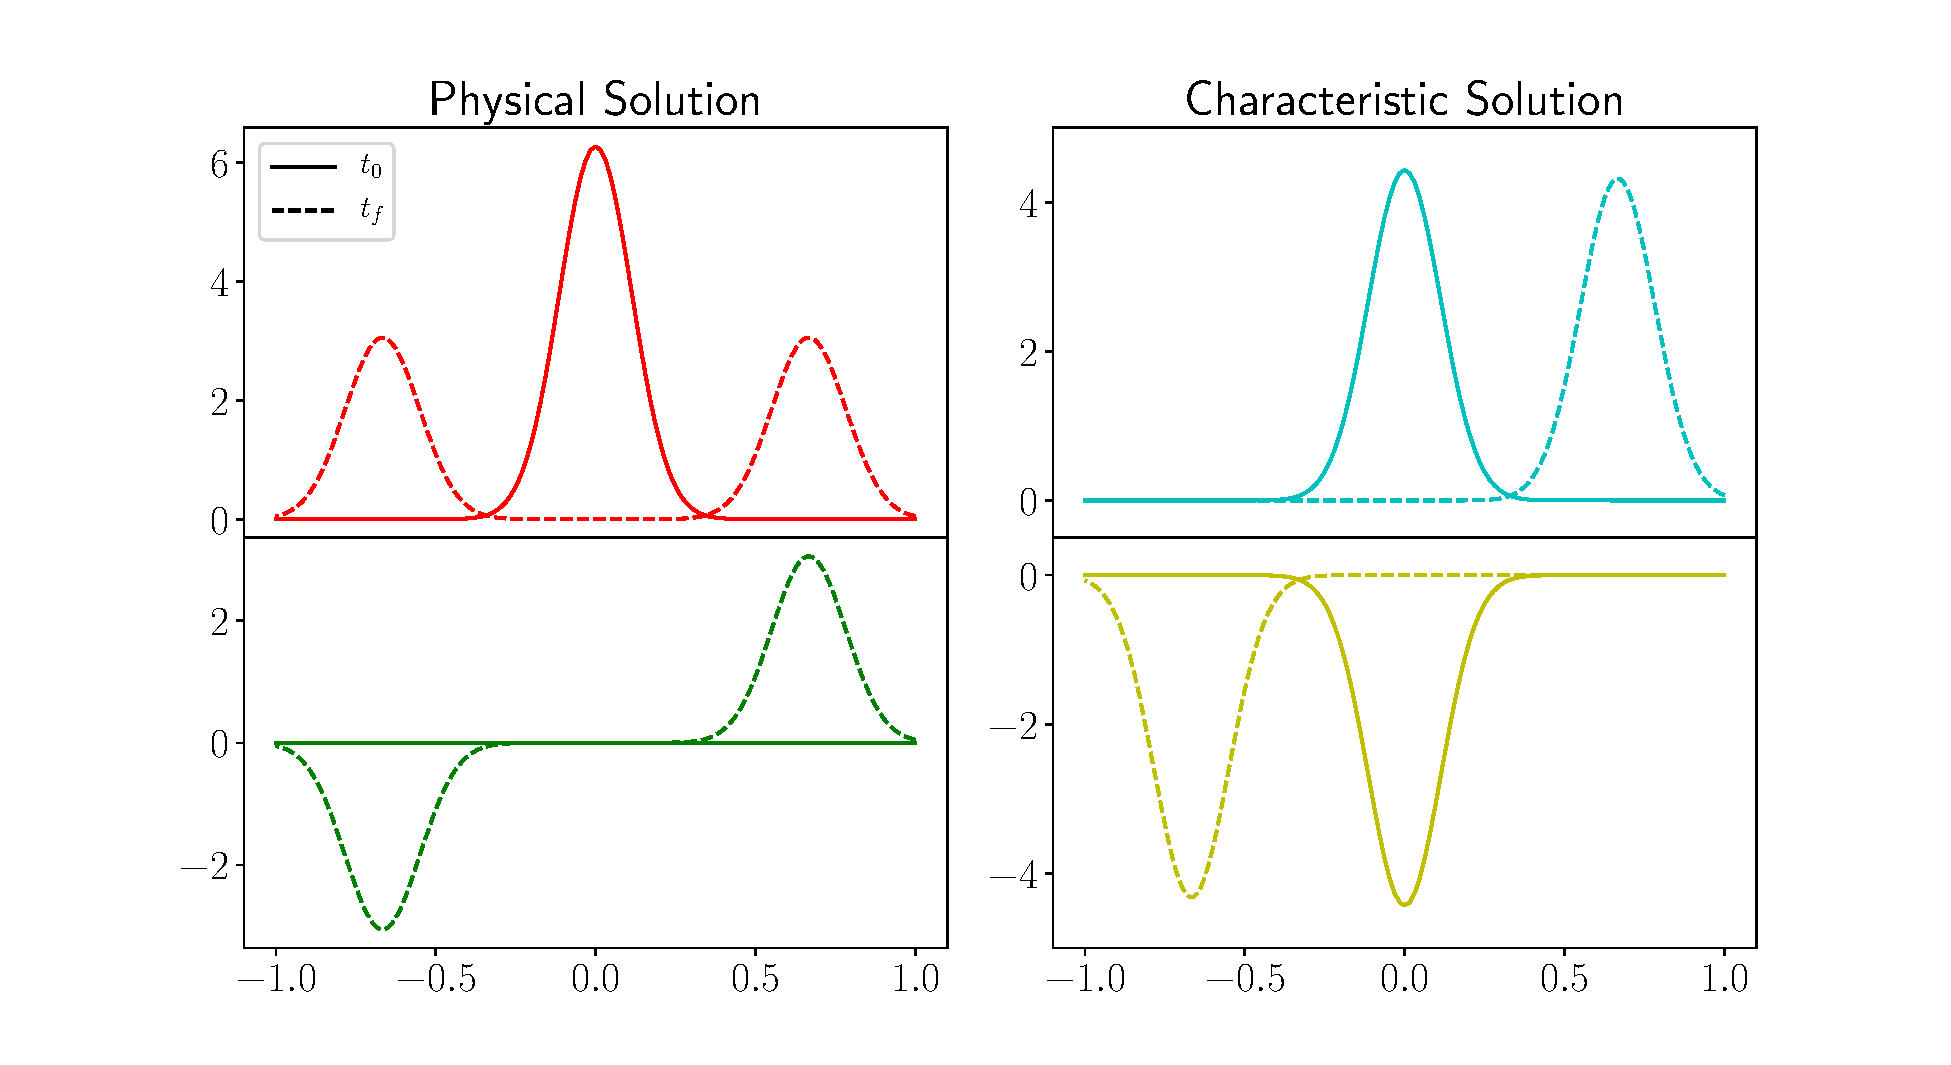
\includegraphics[width=1.25\linewidth]{figures/advection.pdf}
	\end{minipage}
\end{frame}

\section{Results}

\subsection{Examples}

\begin{frame}{Full Example: Wave Equation}
    \makebox[\textwidth][l]{
    \begin{minipage}{\linewidth}
	    \begin{tabular}{m{3cm}m{1.3cm}m{4.5cm}}
	    	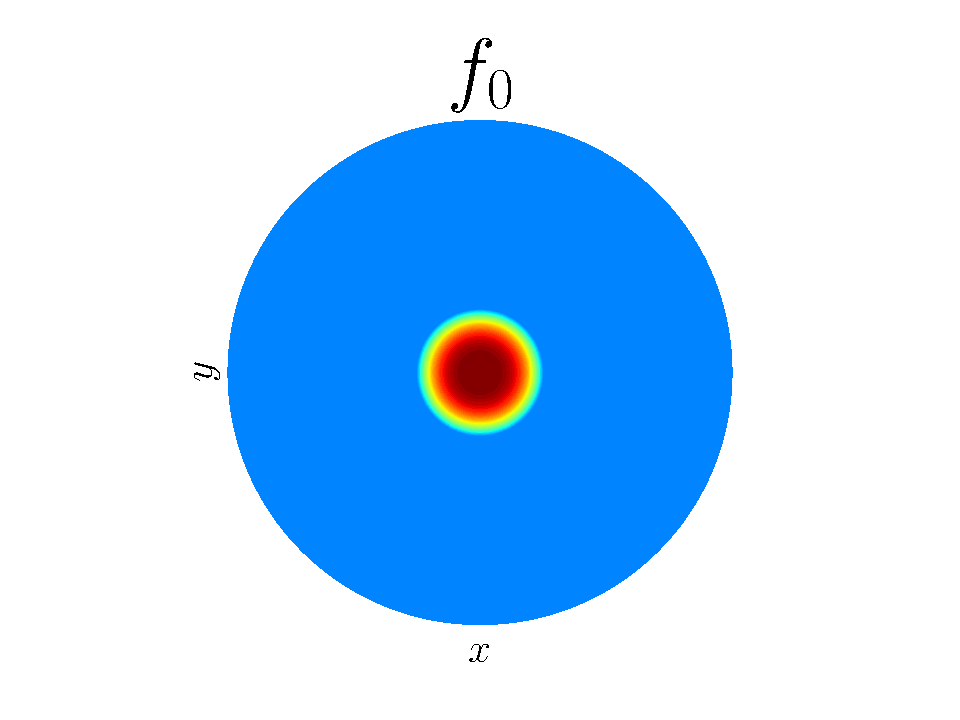
\includegraphics[trim=60 10 80 0, clip,height=3cm]{figures/Physical_Initial.pdf} & $\mathcal{R} \rightarrow $ &  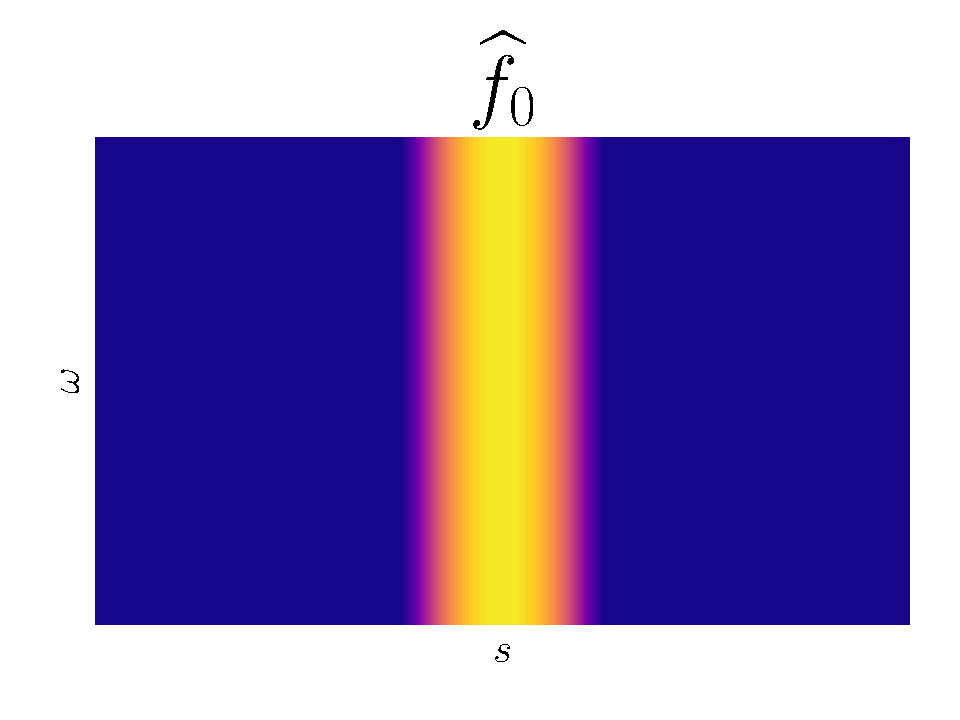
\includegraphics[trim=10 10 0 0, clip,height=3cm]{figures/Radon_Initial.pdf} \\
	    	& &  \small{ $\quad\quad\downarrow$ solve 1D equations } \\
	    	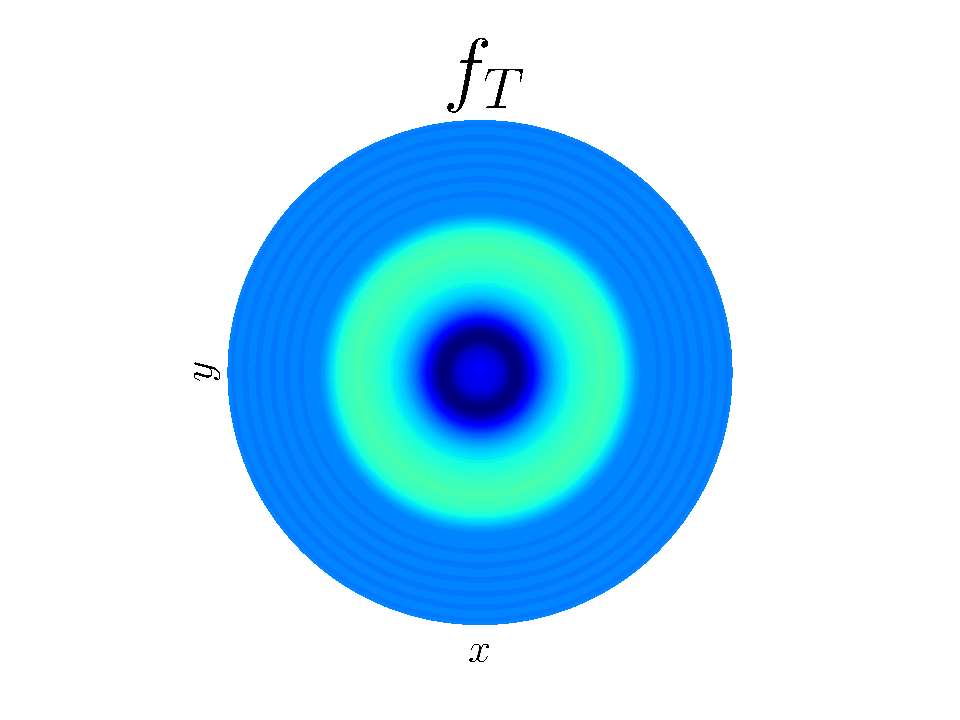
\includegraphics[trim=60 0 80 0, clip,height=3cm]{figures/Physical_Final.pdf} & $\leftarrow \mathcal{R}^{-1}$ &  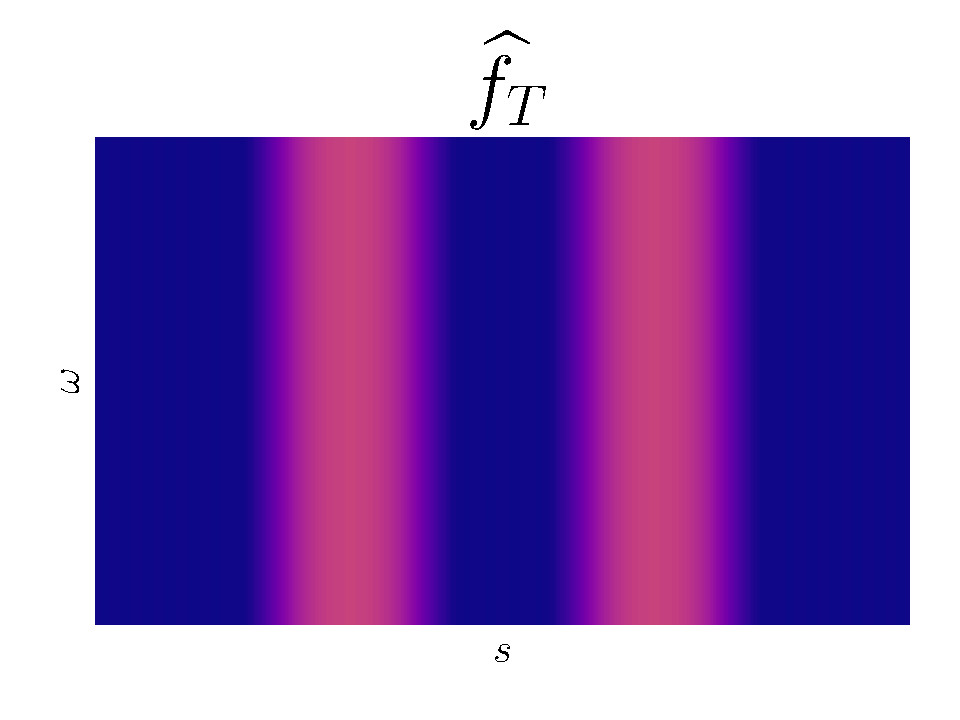
\includegraphics[trim=10 10 0 0, clip,height=3cm]{figures/Radon_Final.pdf}
	    \end{tabular}
     \end{minipage}}
\end{frame}

\begin{frame}{Standard $P_N$ Reference Solution}
    \begin{itemize}
    	\item 
	        In following the standard for testing the $P_N$ equations, we use the following approximate delta function as initial condition with $\alpha = 0.003$
        \begin{align*}
            q_0(x, y) = \frac{1}{4\pi\alpha^2}e^{\frac{ -(x^2 + y^2) }{4\alpha^2} }
            %(1/(4*np.pi*alpha**2))*np.exp(-(((a*x)**2+(a*y)**2)/(4*alpha**2)))
        \end{align*}
        \item 
	        An exact solution to the radially symmetric case can be computed numerically with high accuracy
	    \item
		    Can translate the initial condition and reference solution to test non-symmetric problems
    \end{itemize}
\end{frame}

\begin{frame}{Full Example: $P_1$ Approximation}
    \centering
    \begin{tabular}{>{\centering\arraybackslash}m{5cm} >{\centering\arraybackslash}m{5cm}}
      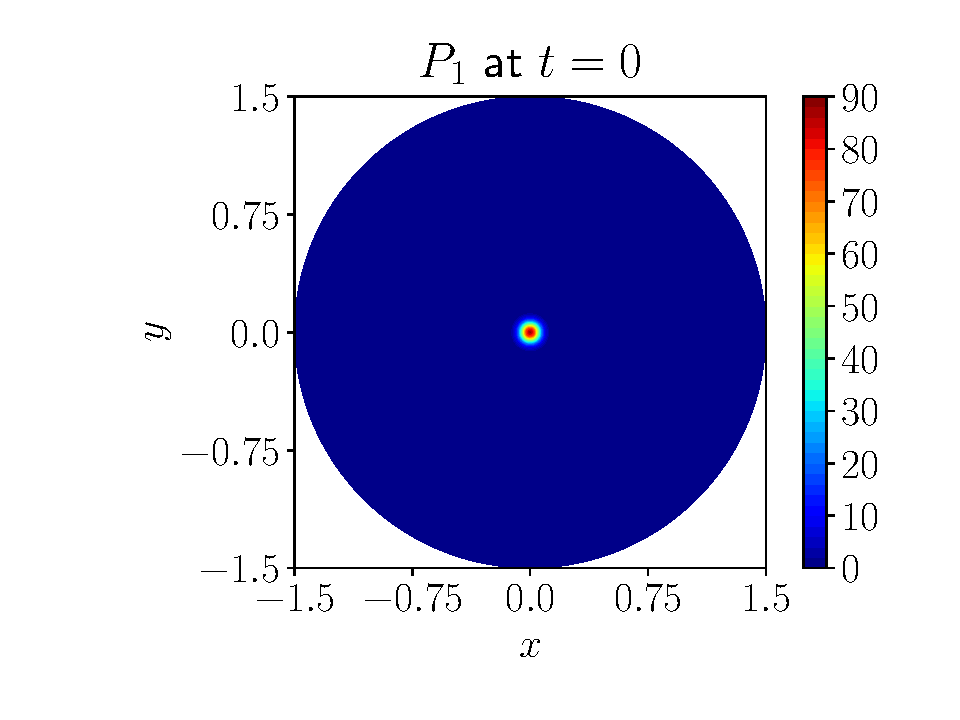
\includegraphics[width=5cm]{figures/physical_initial_p1.pdf} &
      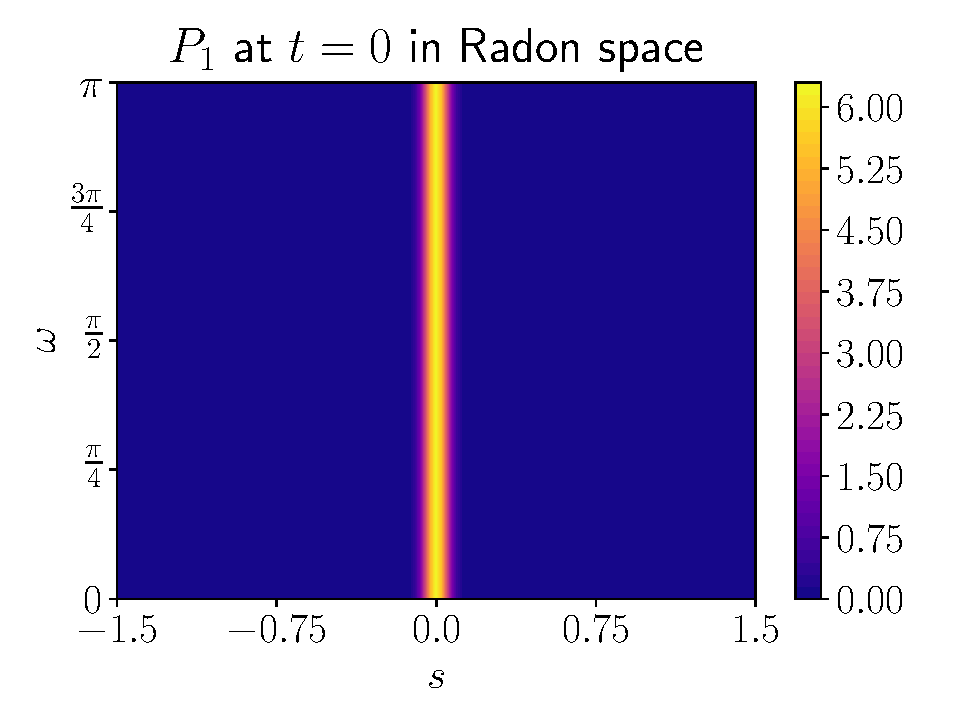
\includegraphics[width=5cm]{figures/radon_initial_p1.pdf} \\
      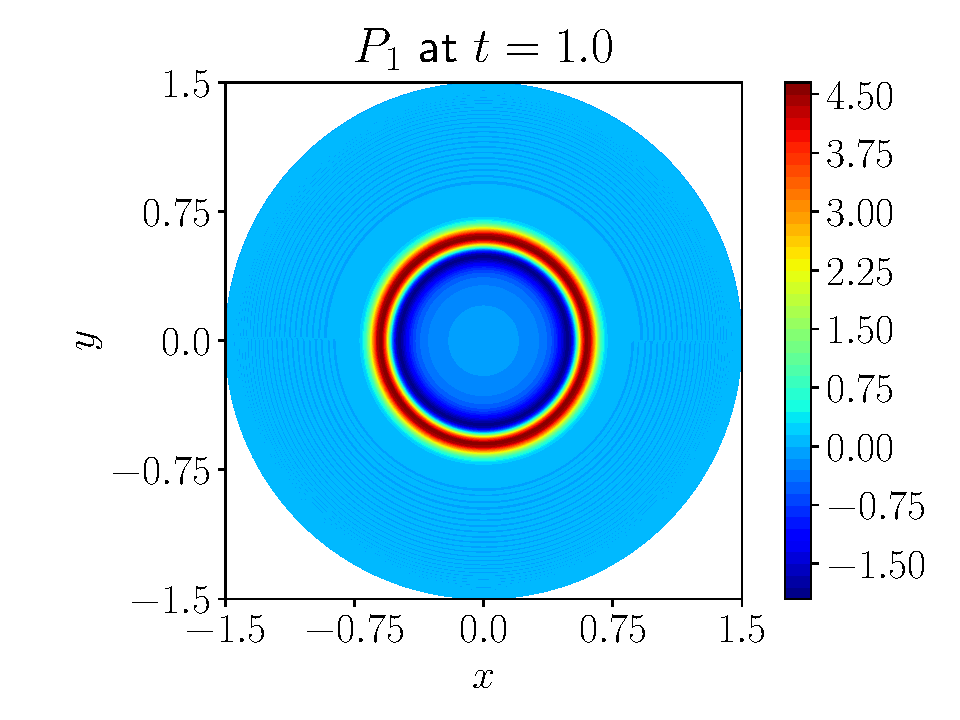
\includegraphics[width=5cm]{figures/physical_final_p1.pdf}  &
      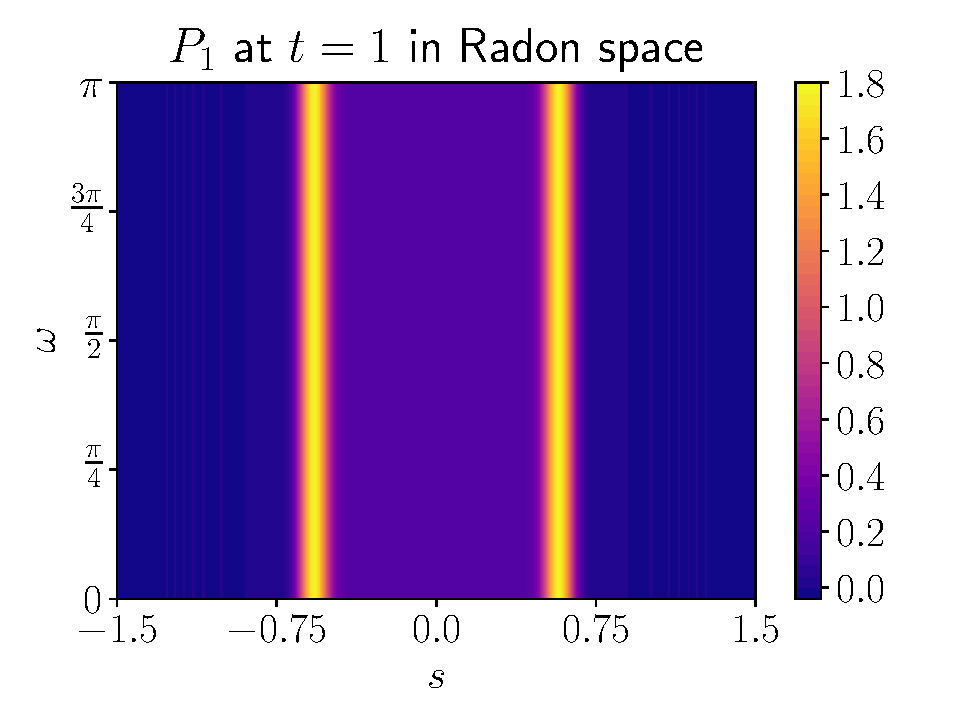
\includegraphics[width=5cm]{figures/radon_final_p1.pdf}
    \end{tabular}
\end{frame}

\begin{frame}{Full Example: $P_1$ Approximation}
    \centering
    \begin{tabular}{>{\centering\arraybackslash}m{5cm} >{\centering\arraybackslash}m{5cm}}
      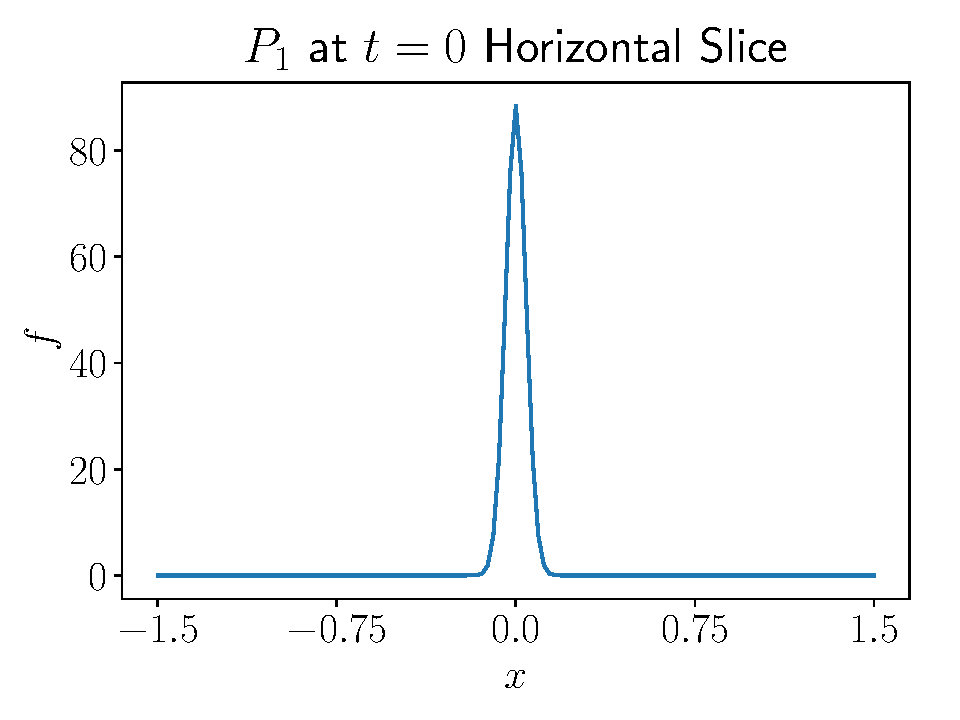
\includegraphics[width=5cm]{figures/Physical_inital_p1_slice.pdf} &
      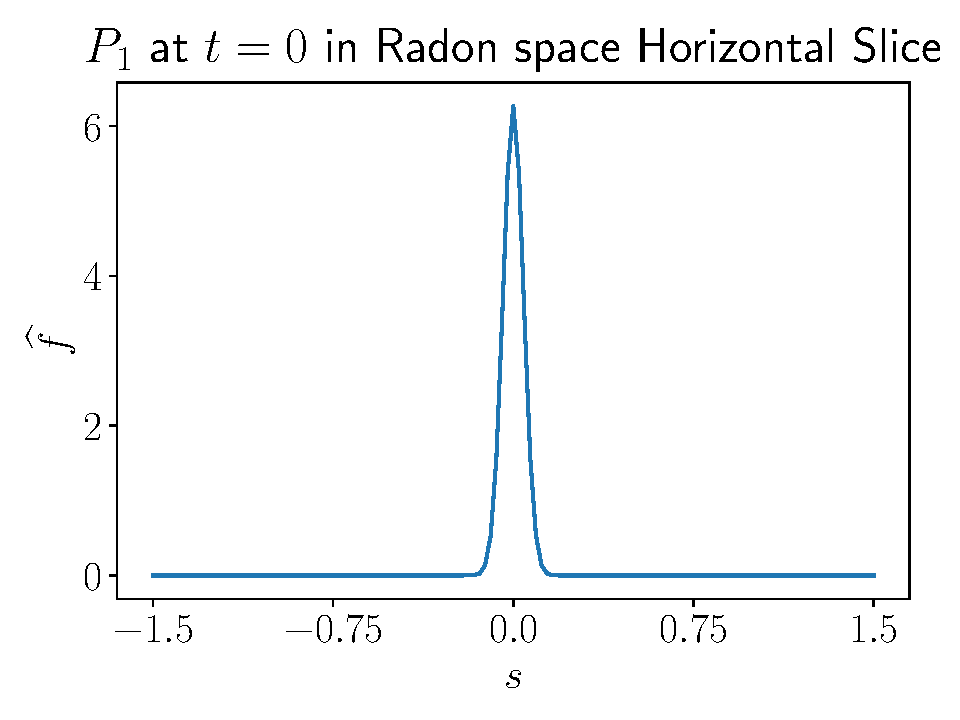
\includegraphics[width=5cm]{figures/radon_inital_p1_slice.pdf} \\
      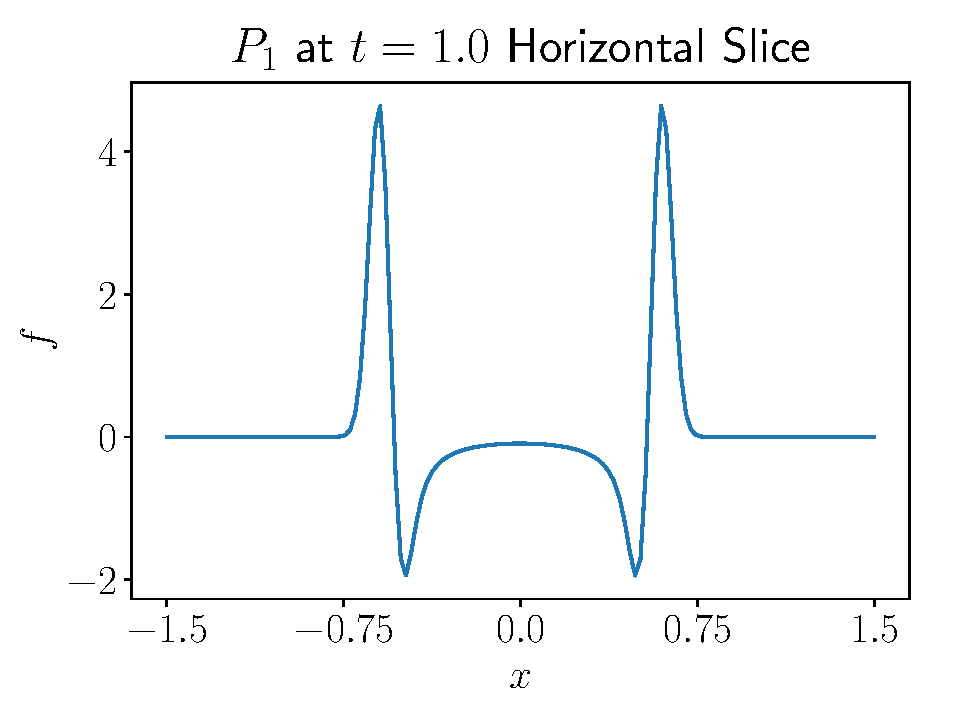
\includegraphics[width=5cm]{figures/Physical_final_p1_slice.pdf}  &
      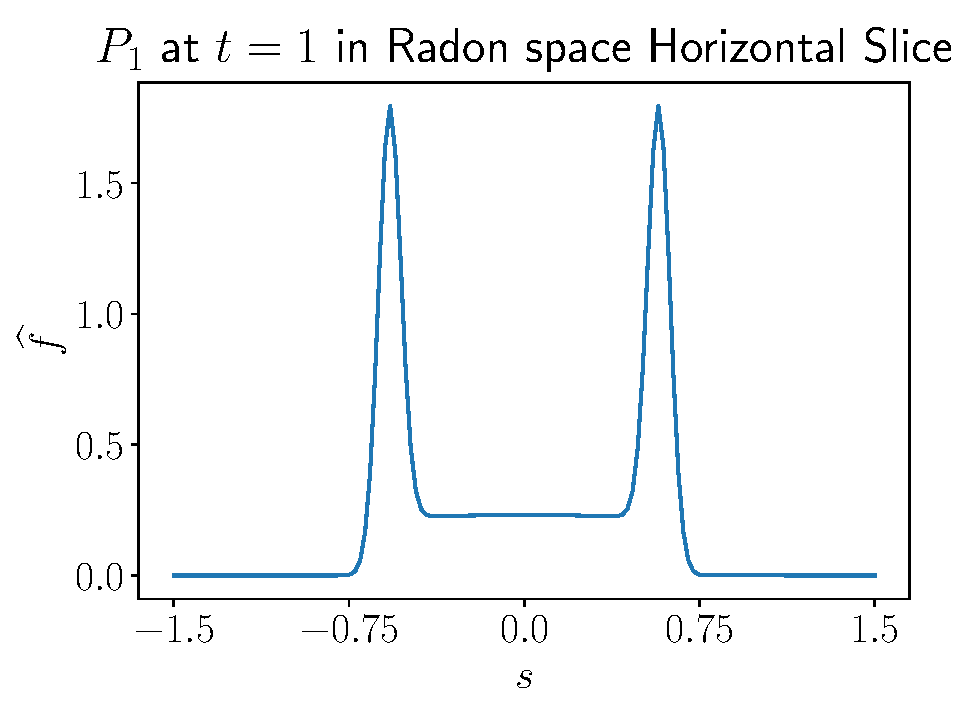
\includegraphics[width=5cm]{figures/radon_final_p1_slice.pdf}
    \end{tabular}
\end{frame}

\subsection{Convergence Studies}

\begin{frame}{Radial Symmetry: Convergence Study on $N_s$}
    \centering
    \begin{itemize}
        \item Radial symmetry means number of angles $N_\omega$ irrelevant
        \item Primary error is in resolving initial condition
    \end{itemize}  
    \centering
    \makebox[\textwidth][l]{                       	
    \hspace{-1cm}
    \begin{minipage}{0.38\linewidth}
    	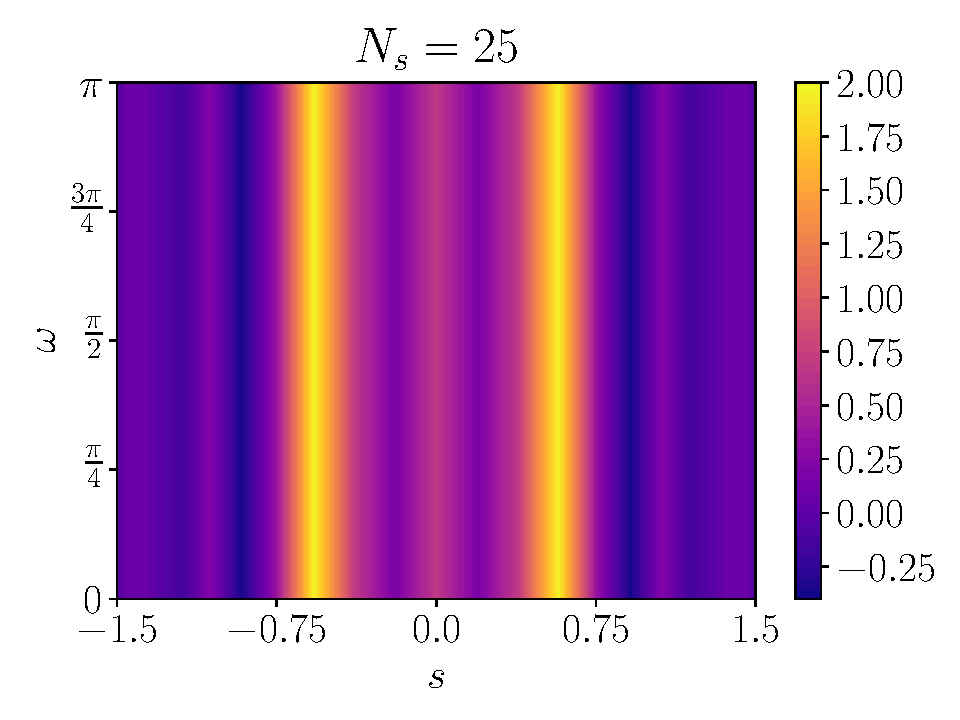
\includegraphics[width=\linewidth]{figures/Radon_Solution_Symmetric_25.pdf} 
	\end{minipage}
	\hspace{-0.25cm}
	\begin{minipage}{0.38\linewidth}
		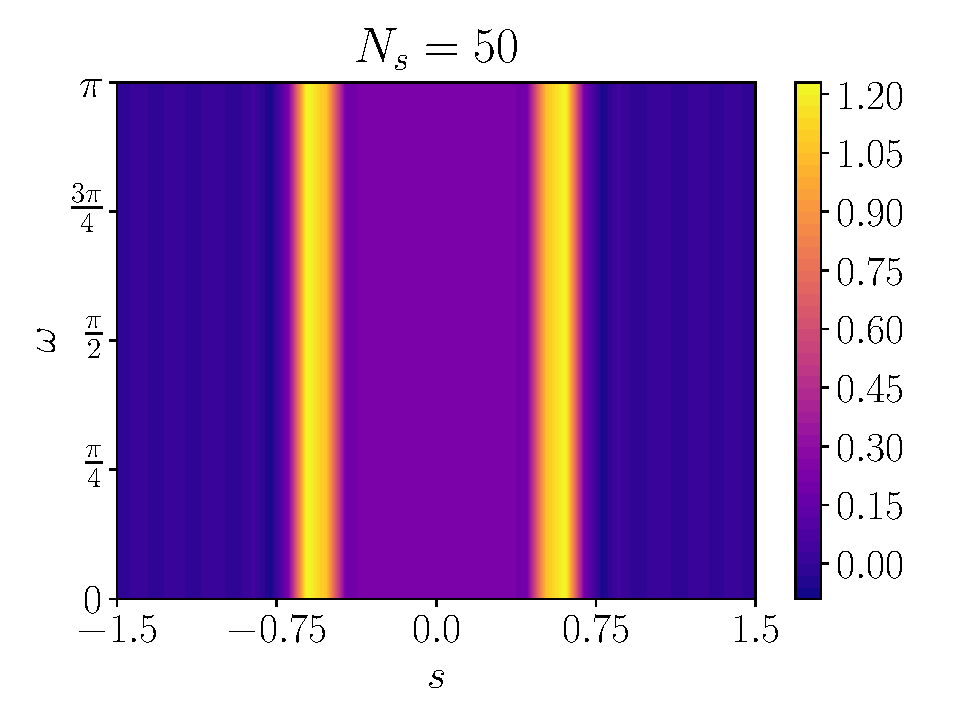
\includegraphics[width=\linewidth]{figures/Radon_Solution_Symmetric_50.pdf} 
	\end{minipage}
	\hspace{-0.25cm}
	\begin{minipage}{0.38\linewidth}
		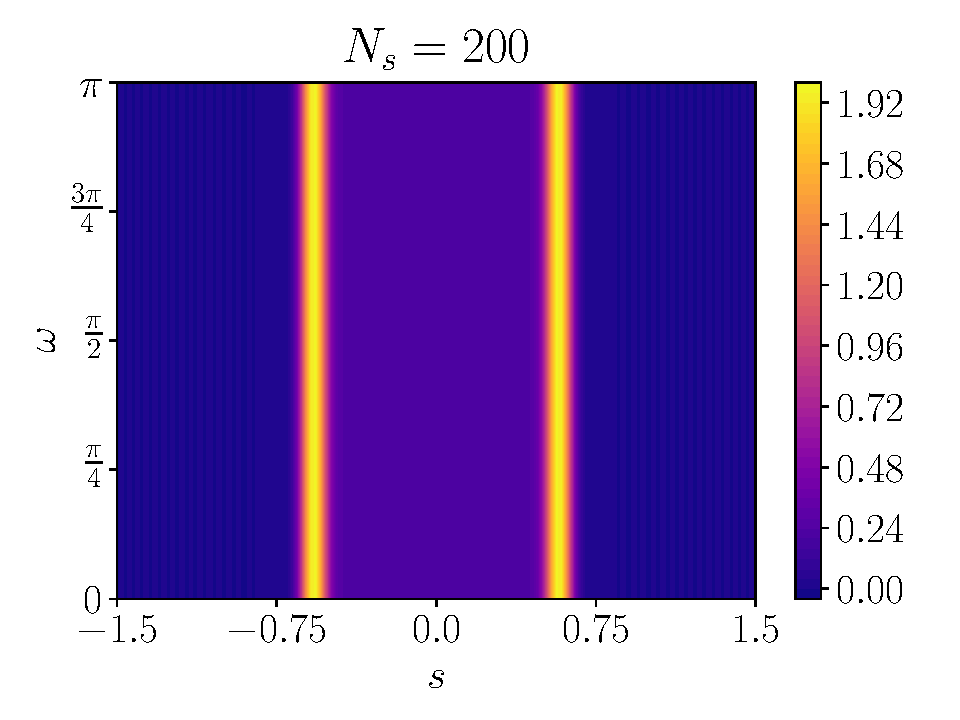
\includegraphics[width=\linewidth]{figures/Radon_Solution_Symmetric_200.pdf} 
	\end{minipage}
	}
\end{frame}

\begin{frame}{Radial Symmetry: Convergence Study on $N_s$}
    \centering
    \makebox[\textwidth][l]{                       	
    \hspace{-1cm}
    \begin{minipage}{0.38\linewidth}
    	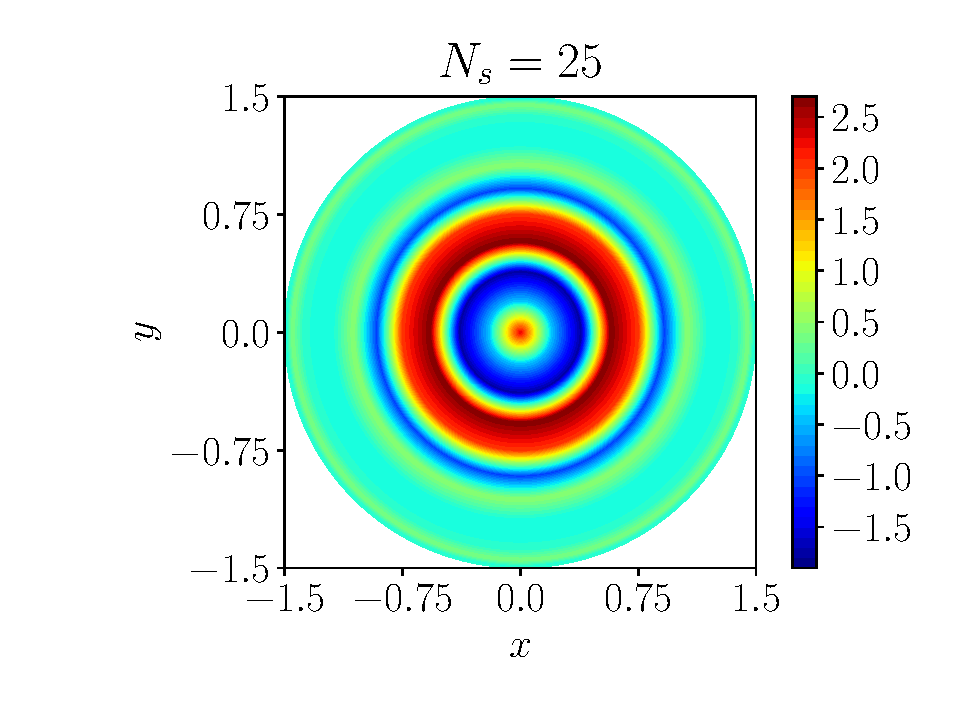
\includegraphics[width=\linewidth]{figures/Physical_Solution_Symmetric_25.pdf} 
	\end{minipage}
	\hspace{-0.25cm}
	\begin{minipage}{0.38\linewidth}
		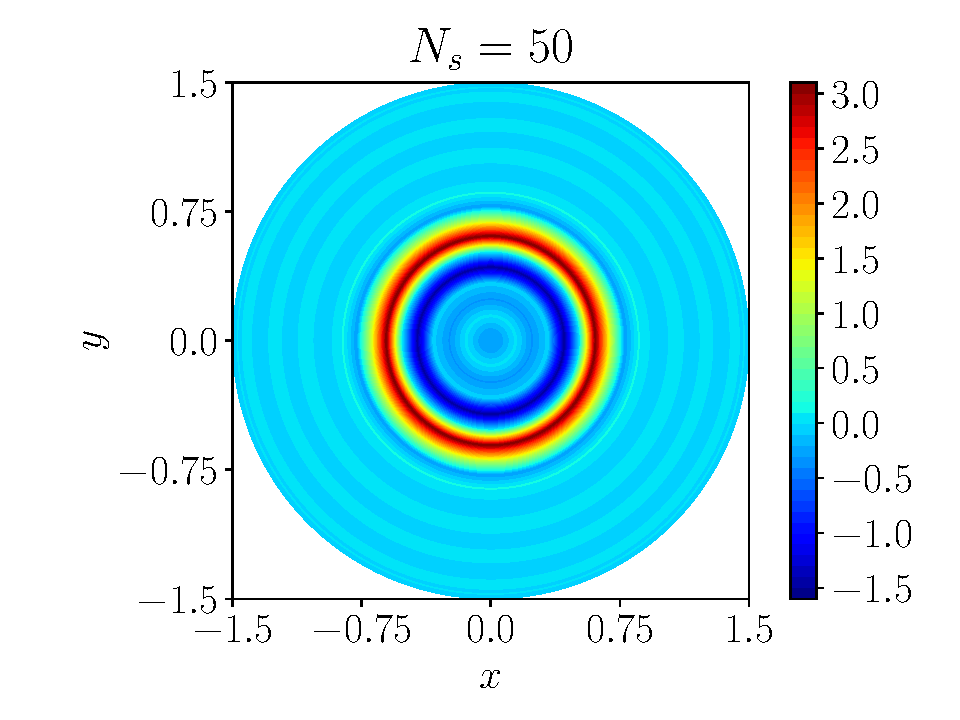
\includegraphics[width=\linewidth]{figures/Physical_Solution_Symmetric_50.pdf} 
	\end{minipage}
	\hspace{-0.25cm}
	\begin{minipage}{0.38\linewidth}
		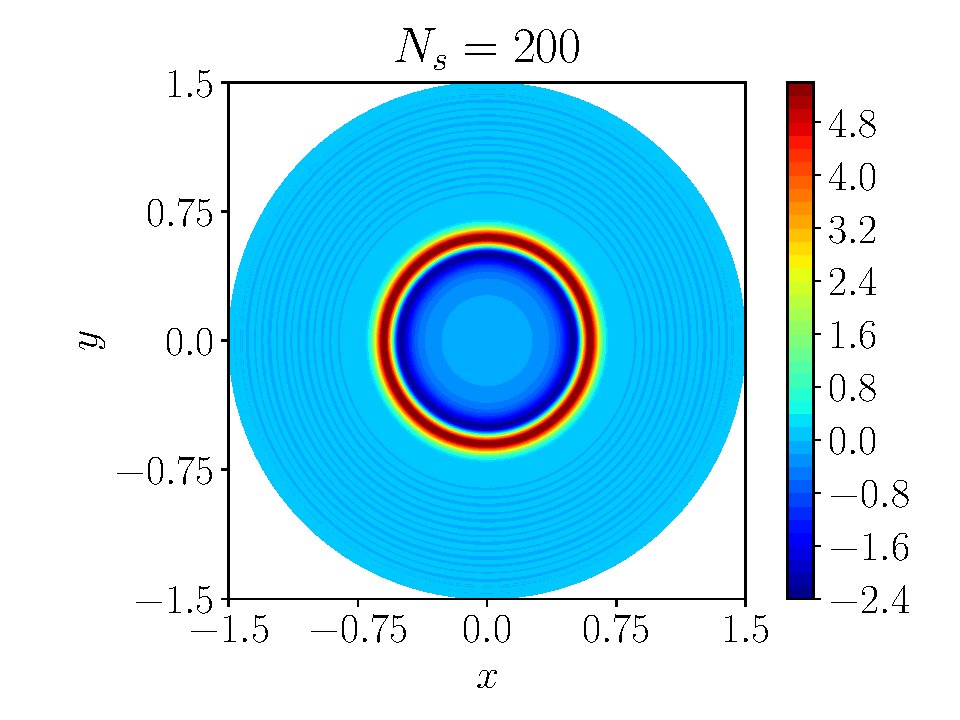
\includegraphics[width=\linewidth]{figures/Physical_Solution_Symmetric_200.pdf} 
	\end{minipage}
	}
	\centering
    \makebox[\textwidth][l]{                       	
    \hspace{-1cm}
    \begin{minipage}{0.38\linewidth}
    	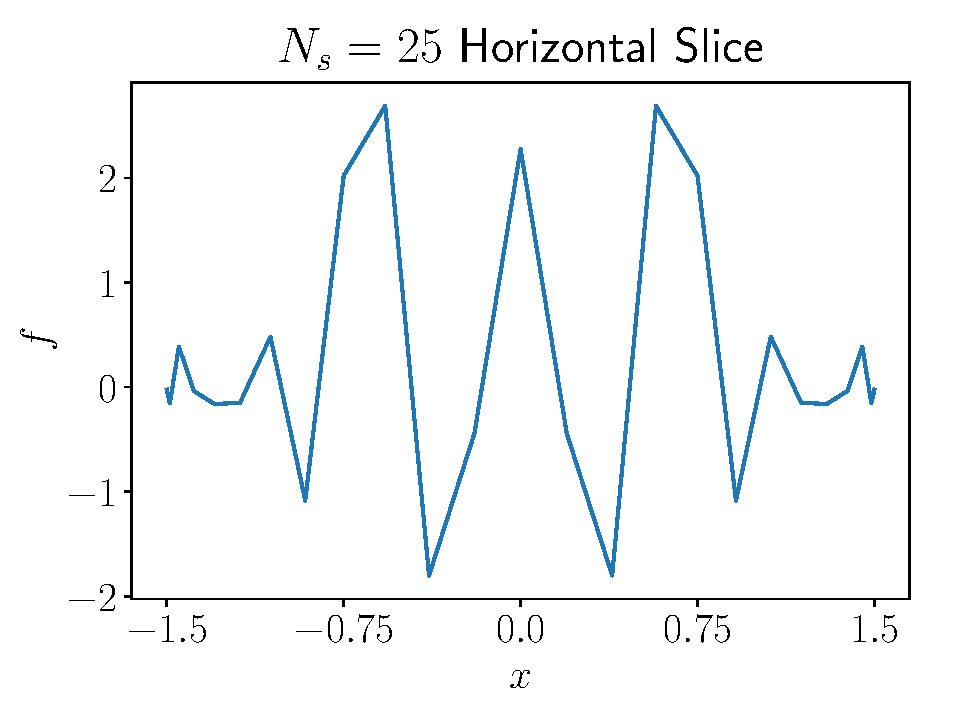
\includegraphics[width=\linewidth]{figures/Physical_Solution_Symmetric_25_slice.pdf} 
	\end{minipage}
	\hspace{-0.25cm}
	\begin{minipage}{0.38\linewidth}
		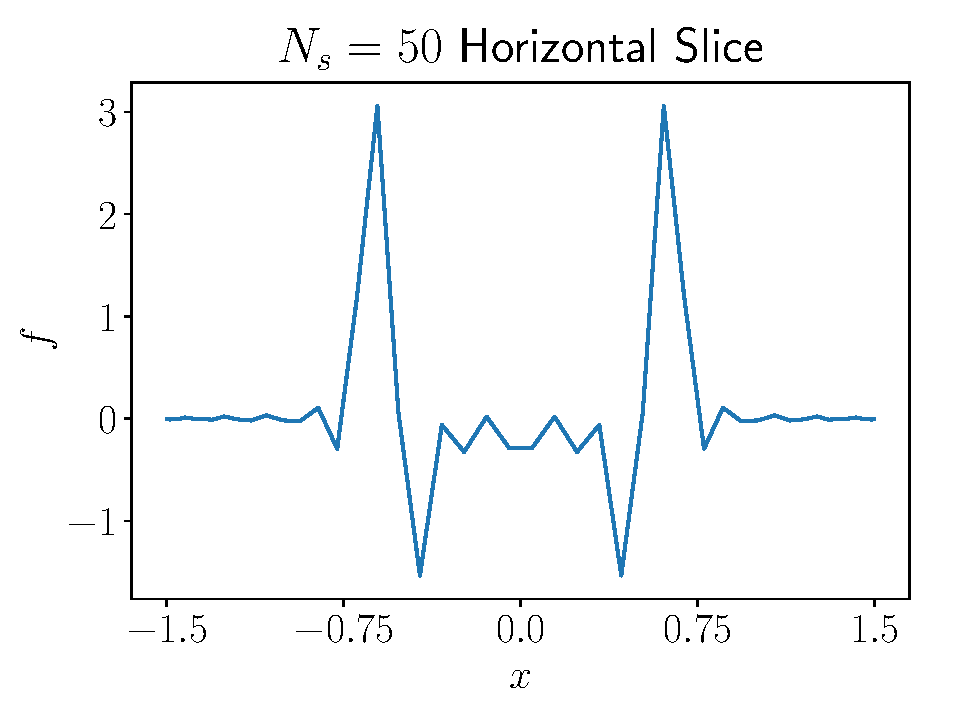
\includegraphics[width=\linewidth]{figures/Physical_Solution_Symmetric_50_slice.pdf} 
	\end{minipage}
	\hspace{-0.25cm}
	\begin{minipage}{0.38\linewidth}
		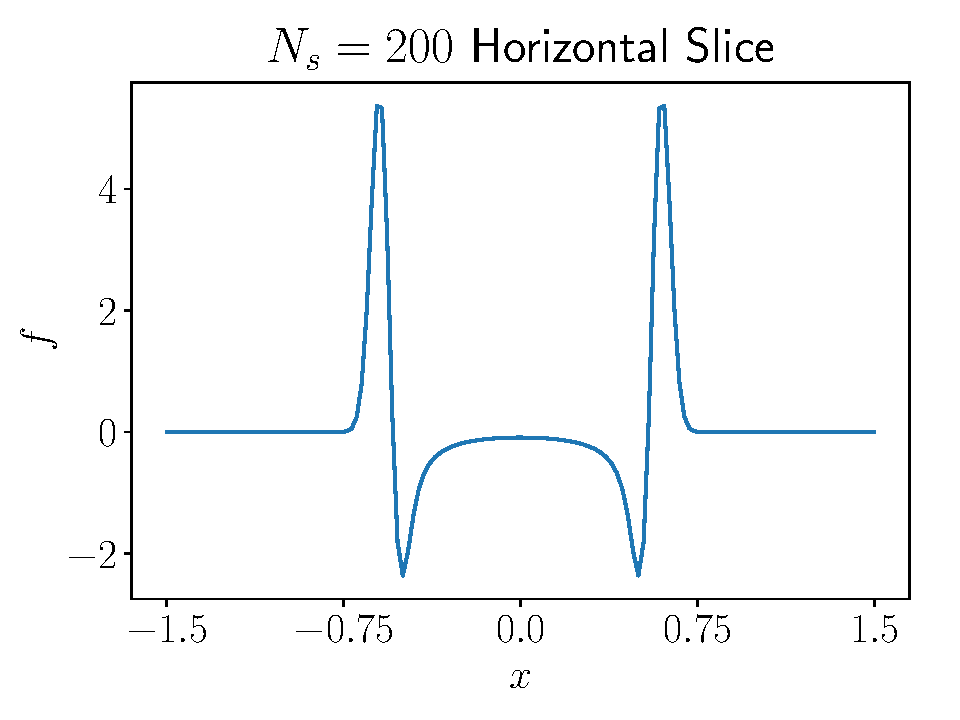
\includegraphics[width=\linewidth]{figures/Physical_Solution_Symmetric_200_slice.pdf} 
	\end{minipage}
	}
\end{frame}

\begin{frame}{Radial Symmetry: Convergence Study on $N_s$}
    \centering
    \hspace{-15mm}
    \makebox[\textwidth][l]{
    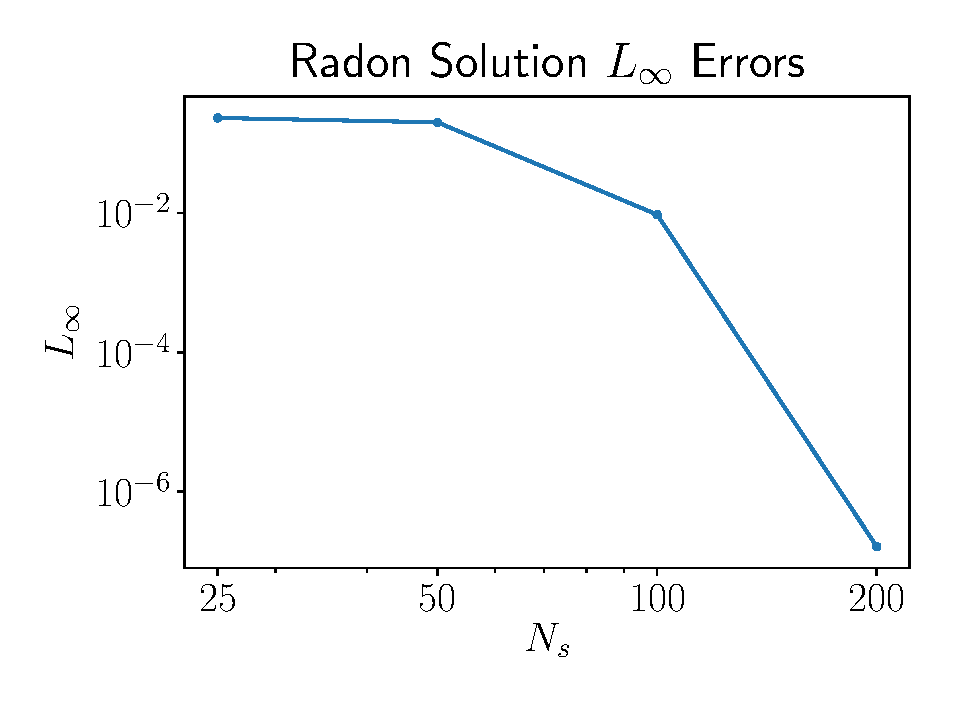
\includegraphics[width=0.55\linewidth]{figures/Convergence_Radon_Errors.pdf}
    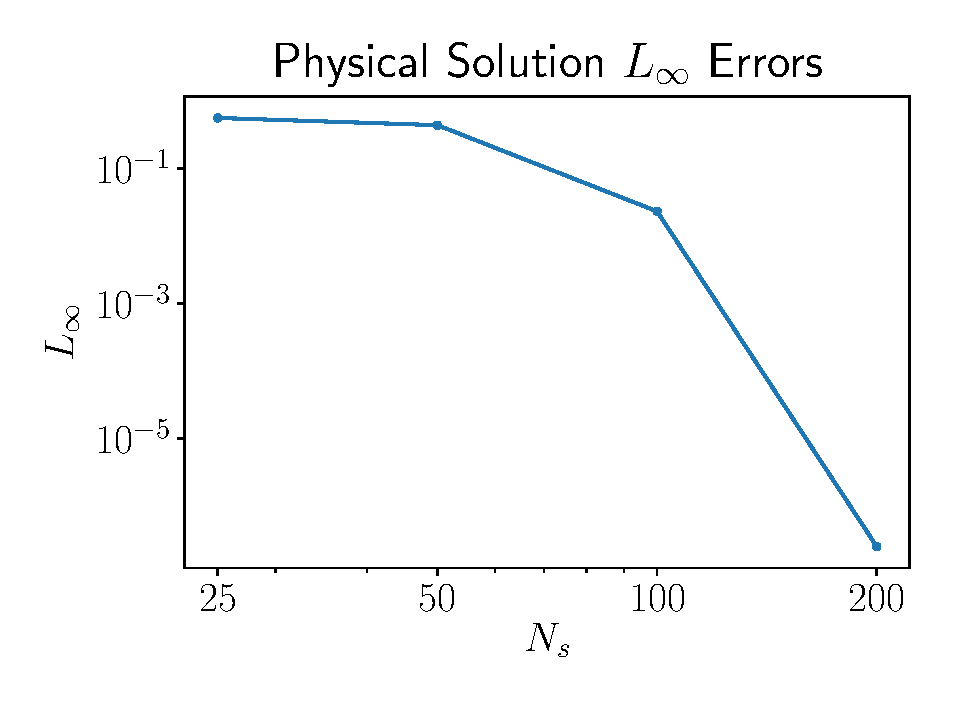
\includegraphics[width=0.55\linewidth]{figures/Convergence_Physical_Errors.pdf}}
    \begin{itemize}
        \item Component methods have varying convergence rates
        \item Solution in Radon space is spectrally accurate in $N_s$
        \item If radially symmetric, spectrally accurate in physical space
    \end{itemize}    
\end{frame}

\begin{frame}{Radial Symmetry: Other $P_N$ Solutions}
    \begin{itemize}
        \item Justified in comparison to existing literature [Shin 2019] due to uniformity of methods across $P_N$
    \end{itemize}
    \centering
    \begin{tabular}{c|c}                    
        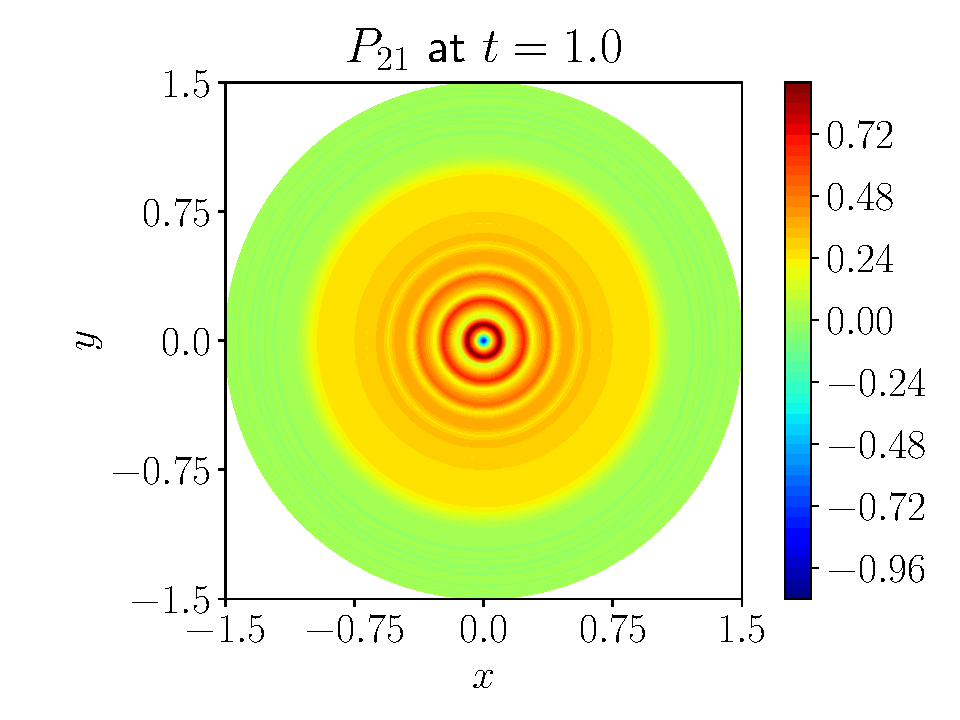
\includegraphics[width=0.35\linewidth]{figures/physical_final_p21.pdf} &
        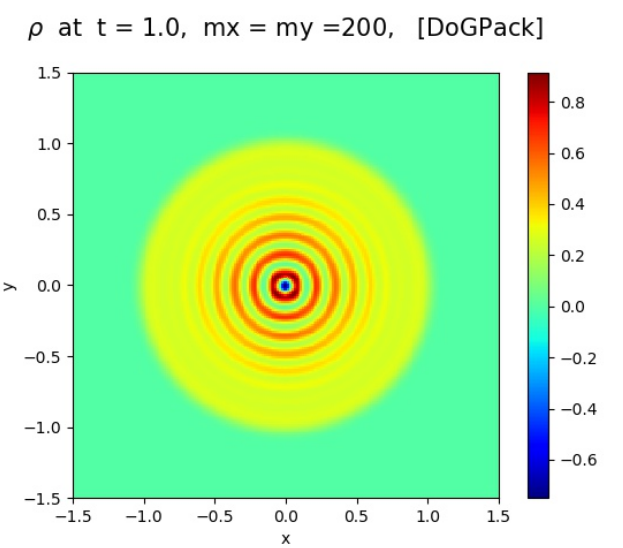
\includegraphics[width=0.3\linewidth]{figures/Minwoo_p21.png} \\
        \includegraphics[width=0.35\linewidth]{figures/physical_final_p41.pdf} &
        \includegraphics[width=0.3\linewidth]{figures/Minwoo_p61.png}
    \end{tabular}
\end{frame}

\begin{frame}{Convergence Study on $N_s$ \quad ($N_\omega = 200$)}
	\centering
	\begin{itemize}
		\item Translating the initial condition disrupts symmetry
		\item Transport step in method independent of symmetry
	\end{itemize}  
	\centering
	\makebox[\textwidth][l]{                       	
		\hspace{-1cm}
		\begin{minipage}{0.38\linewidth}
			\includegraphics[width=\linewidth]{figures/Radon_Solution_Nonsymmetric_25.pdf} 
		\end{minipage}
		\hspace{-0.25cm}
		\begin{minipage}{0.38\linewidth}
			\includegraphics[width=\linewidth]{figures/Radon_Solution_Nonsymmetric_50.pdf} 
		\end{minipage}
		\hspace{-0.25cm}
		\begin{minipage}{0.38\linewidth}
			\includegraphics[width=\linewidth]{figures/Radon_Solution_Nonsymmetric_200.pdf} 
		\end{minipage}
	}
\end{frame}

\begin{frame}{Convergence Study on $N_s$ \quad ($N_\omega = 200$)}
    \centering
    \makebox[\textwidth][l]{                       	
    \hspace{-1cm}
    \begin{minipage}{0.38\linewidth}
    	\includegraphics[width=\linewidth]{figures/Physical_Solution_Nonsymmetric_25_Ns.pdf} 
	\end{minipage}
	\hspace{-0.25cm}
	\begin{minipage}{0.38\linewidth}
		\includegraphics[width=\linewidth]{figures/Physical_Solution_Nonsymmetric_50_Ns.pdf} 
	\end{minipage}
	\hspace{-0.25cm}
	\begin{minipage}{0.38\linewidth}
		\includegraphics[width=\linewidth]{figures/Physical_Solution_Nonsymmetric_200_Ns.pdf} 
	\end{minipage}
	}
	\centering
    \makebox[\textwidth][l]{                       	
    \hspace{-1cm}
    \begin{minipage}{0.38\linewidth}
    	\includegraphics[width=\linewidth]{figures/Physical_Solution_Nonsymmetric_25_slice_Ns.pdf} 
	\end{minipage}
	\hspace{-0.25cm}
	\begin{minipage}{0.38\linewidth}
		\includegraphics[width=\linewidth]{figures/Physical_Solution_Nonsymmetric_50_slice_Ns.pdf} 
	\end{minipage}
	\hspace{-0.25cm}
	\begin{minipage}{0.38\linewidth}
		\includegraphics[width=\linewidth]{figures/Physical_Solution_Nonsymmetric_200_slice_Ns.pdf} 
	\end{minipage}
	}
\end{frame}

\begin{frame}{Convergence Study on $N_s$ \quad ($N_\omega = 200$)}
	\centering
    \hspace{-15mm}
    \makebox[\textwidth][l]{
	\includegraphics[width=0.55\linewidth]{figures/Convergence_Radon_Errors_Ns.pdf}
    \includegraphics[width=0.55\linewidth]{figures/Convergence_Physical_Errors_Ns.pdf}}
	\begin{itemize}
		\item $N_s$ indirectly affects convergence of physical solution
	\end{itemize}    
\end{frame}

\begin{frame}{Convergence Study on $N_\omega$ \quad ($N_s = 200$)}
	\centering
	\begin{itemize}
		\item Need to consider effect of angular discretization seperately
		\item Solving each 1D system is independent of choice of $N_\omega$
	\end{itemize}  
	\centering
	\makebox[\textwidth][l]{                       	
		\hspace{-1.5cm}
		\begin{minipage}{0.43\linewidth}
			\includegraphics[width=\linewidth]{figures/Physical_Solution_Nonsymmetric_25.pdf} 
		\end{minipage}
		\hspace{-0.45cm}
		\begin{minipage}{0.41\linewidth}
			\includegraphics[width=\linewidth]{figures/Physical_Solution_Nonsymmetric_50.pdf} 
		\end{minipage}
		\hspace{-0.45cm}
		\begin{minipage}{0.41\linewidth}
			\includegraphics[width=\linewidth]{figures/Physical_Solution_Nonsymmetric_200.pdf} 
		\end{minipage}
	}
\end{frame}

\begin{frame}{Convergence Study on $N_\omega$ ($N_s = 200$)}
	\centering
	\includegraphics[width=0.6\linewidth]{figures/Convergence_Physical_Errors_Nw.pdf}
	\begin{itemize}
		\item Transport step identical across tests
		\item Interpolation across anges is 4th order
	\end{itemize}    
\end{frame}

\begin{frame}{Nonsymmetric: Other $P_N$ examples}
    \begin{itemize}
        \item Primary source of instability is singularity at the origin
    \end{itemize}
    \centering
	\begin{tabular}{c|c}
 	    \includegraphics[width=0.35\linewidth]{figures/physical_final_p7_shift.pdf} &
    	\includegraphics[width=0.3\linewidth]{figures/Minwoo_p7.png} \\
    	\includegraphics[width=0.35\linewidth]{figures/physical_final_p21_shift.pdf} &
    	\includegraphics[width=0.3\linewidth]{figures/Minwoo_p21.png}
    \end{tabular}
\end{frame}

\subsection*{Summary}

\begin{frame}{Summary}
    \begin{itemize}
        \item
            Use the forward Radon transform on a linear system of hyperbolic PDEs
        \item
            Solve each system in the collection of 1D transport equations
        \item
            Use the inverse Radon transform to bring solution back to physical space
  \end{itemize}
\end{frame}

\begin{frame}{Acknowledgments}
\begin{itemize}
    \item
        NSF Grant DMS-1457443
    \item
        Iowa State University
    \item
        Dr. Rossmanith
    \item
        Christine Wiersma
\end{itemize}
\end{frame}

\begin{frame}{Thank You!}
    \begin{itemize}
        \item
            Future Work
        \begin{itemize}
            \item
                Adding spatially-dependent collision terms to the $P_N$ equations
            \item 
                Implementing more sophisticated/higher order timestepping schemes
            \item
                Improving efficiency through a parallelization of transport computations
            \\ \color{white} hi \color{black} \\ %puts a space so the slide fills up more
        \end{itemize}
        \pause
        \item
            Questions?
    \end{itemize}
\end{frame}

\begin{frame}{References}
    (1) Brunner, T. \& Holloway, J. (2005). \textit{Two-dimensional time dependent Riemann solvers for neutron transport}, Journal of Computational Physics 210 (2005) 386-399. 
        \\ \color{white} hi \color{black} \\
    (2) Peterson, L. (2018). \textit{An asymptotic-preserving spectral method based on the radon transform for the PN approximation of radiative transfer}, Master's thesis, Iowa State University, 2018. 
        \\ \color{white} hi \color{black} \\
    (3) Pieraccini, S. \& Puppo, G. (2007). \textit{Implicit-Explicit Schemes for BGK Kinetic Equations}, Journal of Scientific Computing, Vol. 32, No. 1, July 2007.
\end{frame}

\begin{frame}{References (cont.)}
    (4) Press, W. (2006). \textit{Discrete Radon transform has an exact, fast inverse and generalizes to operations other than sums along lines}, PNAS December 19, 2006 103 (51) 19249-19254
        \\ \color{white} hi \color{black} \\
    (5) Rim, D. (2018). \textit{Dimensional splitting of hyperbolic partial differential equations using the Radon transform}, SIAM J. Sci. Comput., 40(6) (2018), A4184-A4207
        \\ \color{white} hi \color{black} \\
    (6) Shin, M. (2019). \textit{Hybrid discrete ($H^T_N$) approximations to the equation of radiative transfer}, Ph.D. thesis, Iowa State University, 2019.
        \\ \color{white} hi \color{black} \\
    (7) Trefethen, L. (2000). \textit{Spectral Methods in MATLAB}, Society for Industrial and Applied Mathematics, 2000.
\end{frame}

\section*{Glossary of Numerical Methods}
\begin{frame}{Clenshaw-Curtis Quadrature}
    \begin{itemize}
        \item Let $\tau$ be half the length of the chord perpendicular to $(s, \omega)$
        \begin{align*}
        	& \int_{-\tau}^{\tau} f(s_{i} \cos (\omega_{j}) - z \sin (\omega_{j}), \, s_{i} \sin (\omega_{j}) + z \cos (\omega_{j})) \, dz \\
        	= \, & \tau \int_{-1}^{1} f(s_{i} \cos (\omega_{j}) - \tau t \sin (\omega_{j}), \, s_{i} \sin (\omega_{j}) + \tau t \cos (\omega_{j})) \, dt \\
            \approx \, & \tau \sum_{k=0}^{N_q} w_{k} \, f(s_{i} \cos (\omega_{j}) - \tau t_{k} \sin (\omega_{j}), \, s_{i} \sin (\omega_{j}) + \tau t_{k} \cos (\omega_{j}))
        \end{align*}
    where $t_k$ are Chebyshev points of the second kind in $[-1, 1]$
    \end{itemize}
\end{frame}

\begin{frame}{Barycentric Interpolation}
\begin{itemize}
    \item
        Stabilized barycentric interpolation formula:
\begin{align*}
    H_n(x)&= \frac{\sum_{j = 0}^{n} \alpha_j \frac{f_j}{x-x_j}}{\sum_{j = 0}^{n} \alpha_j\frac{1}{x-x_j}} \\ 
    \alpha_0 = \frac{1}{2},\quad \alpha_{1:n-1} = &(-1)^{1:n-1},\quad \alpha_n = \frac{1}{2} (-1)^n \\
\end{align*} 
\end{itemize}
\end{frame}

\begin{frame}{4 Point Polynomial Interpolation}
\begin{itemize}
    \item
        Let $\theta_0$ be the midpoint of the arc containing $h_i$, $i=1,\dots,4$ 
\begin{align*}
    p(\theta) = - &\frac{1}{16}(h_1 - 9h_2 - 9h_3 + h_4) \\
    + &\frac{1}{24d\omega}(h_1 - 27h_2 + 27h_3 - h_4)(\theta - \theta_0) \\
    + &\frac{1}{4d\omega^2}(h_1 - h_2 - h_3 + h_4)(\theta - \theta_0)^2 \\
    - &\frac{1}{6d\omega^3}(h_1 - 3h_2 + 3h_3 - h_4)(\theta - \theta_0)^3
\end{align*}
\end{itemize}
\end{frame}

\begin{frame}{Spectral Differentiation Matrix}
    \centering
    \includegraphics[width=0.8\textwidth]{figures/Chebyshev.jpg}
\end{frame}

\begin{frame}{Boundary Conditions}
\begin{itemize}
    \item
        Sign of $\lambda_p$ determines direction of inflow. 
    \item Negative $\implies$ left
        
    \begin{minipage}[c]{0.5\linewidth}
      \[
        \mat{D}_{\,\text{left}} = \left[
        \begin{array}{c|cc}
          0 & \dots & 0 \\ \hline
          \vdots & \ddots &  \\
          0 & & D
        \end{array}
        \right]
      \]
    \end{minipage}
    \begin{minipage}[c]{0.4\linewidth}
      \[
        \mat{D}_{\,\text{right}} = \left[
        \begin{array}{cc|c}
          D &  & 0 \\ 
            & \ddots & \vdots \\\hline
          0 & \dots & 0
        \end{array}
        \right]
      \]
    \end{minipage}
\end{itemize}
\end{frame}

\begin{frame}{IMEX Method Butcher Tableu}
    \begin{small}
    	\begin{minipage}[c]{0.5\linewidth}
    		\[\arraycolsep=2.5pt\def\arraystretch{1.2}
    		\begin{array}{c|c}
    		\tilde{c} & \tilde{A} \\ \hline
    		& \tilde{w} \\
    		\end{array}
    		=
    		\begin{array}{c|cccc}
    		0 & 0 &  &  &  \\
    		0 & 0 & 0 &  &  \\
    		1 & 0 & 1 & 0 &  \\
    		\frac{1}{2} & 0 & \frac{1}{4} & \frac{1}{4} & 0 \\ \hline
    		& 0 & \frac{1}{6} & \frac{1}{6} & \frac{2}{3}
    		\end{array}
    		\]
    	\end{minipage}
    	\begin{minipage}[c]{0.4\linewidth}
    		\[\arraycolsep=2.5pt\def\arraystretch{1.2}
    		\begin{array}{c|c}
    		c & A \\ \hline
    		& w \\
    		\end{array}
    		=
    		\begin{array}{c|cccc}
    		\alpha & \alpha &  &  &  \\
    		0 & -\alpha & \alpha &  &  \\
    		1 & 0 & 1-\alpha & \alpha &  \\
    		\frac{1}{2} & \beta & \eta & \frac{1}{2} - \beta - \eta & \alpha \\ \hline
    		& 0 & \frac{1}{6} & \frac{1}{6} & \frac{2}{3}
    		\end{array}
    		\]
    	\end{minipage}
    \end{small}
\end{frame}

\begin{frame}{3rd-Order IMEX}
	\begin{itemize}
		\item
		Each stage must be computed for $p=1, \dots, M$
	\end{itemize}
	\begin{align*}
	&w^{ \, (1)}_p = w^{ \, k}_p - {\Delta t} \, a_{11} \, \lambda_p \, w^{ \, (1)}_{p,s}, \\ 
	&\text{for $i = 2,\dots,\nu$}\\
	&\quad w^{ \, (i)}_p = w^{ \, k}_p + \Delta t \sum_{\ell = 1}^{i-1} \tilde{a}_{i\ell} \, \sum_{q=1}^M F_{pq} \, w^{ \, (\ell)}_q - {\Delta t} \sum_{\ell=1}^{i} a_{i\ell} \, \lambda_p \, w^{(\ell)}_{p,s} \\
	&w_p^{ \, k+1} = w^{ \, k}_p + \Delta t \sum_{i=1}^{\nu} \tilde{w}_i \, \sum_{q=1}^M F_{pq} \, w^{ \, (i)}_q - {\Delta t} \sum_{i = 1}^{\nu} w_i \, \lambda_p \, w^{ \, (i)}_{p,s}
	\end{align*}
\end{frame}

\begin{frame}{Reference Solution PDE}
	\begin{itemize}
		\item The following coupled PDE in physical space governs the $P_{1}$ approximation with radially symmetric initial conditions
		\begin{align*}
		\begin{bmatrix}
		p \\
		u_{r}
		\end{bmatrix}_{, t} + 
		\begin{bmatrix}
		0 & \frac{1}{\sqrt{3}} \\
		\frac{1}{\sqrt{3}} & 0
		\end{bmatrix}
		\begin{bmatrix}
		p \\
		u_{r}
		\end{bmatrix}_{, r} = 
		\begin{bmatrix}
		-\frac{1}{\sqrt{3}} \frac{1}{r} u_{r} \\
		-\sigma u_{r}
		\end{bmatrix}
		\end{align*}
		\item Can rewrite in characteristic variables and solve exactly
		\item Run with high  resolution ($N_s = N_\omega = 400$) to use in convergence studies
	\end{itemize}    
\end{frame}

\end{document}




